\documentclass[12pt, oneside]{article}   	% use "amsart" instead of "article" for AMSLaTeX format
\usepackage{geometry}                		% See geometry.pdf to learn the layout options. There are lots.
\geometry{letterpaper}                   		% ... or a4paper or a5paper or ... 
%\geometry{landscape}                		% Activate for for rotated page geometry
%\usepackage[parfill]{parskip}    		% Activate to begin paragraphs with an empty line rather than an indent
\usepackage{graphicx}				% Use pdf, png, jpg, or eps� with pdflatex; use eps in DVI mode
\usepackage{amsmath}
\usepackage{mathtools}
								% TeX will automatically convert eps --> pdf in pdflatex		
\usepackage{amssymb}
\numberwithin{equation}{section}
\numberwithin{table}{section}
\usepackage{color}
\usepackage[toc,page]{appendix}
\usepackage[hypcap]{caption}
\usepackage{caption}
\usepackage{glossaries}
\usepackage{commath}
\usepackage{float}
\usepackage{pbox}
%\usepackage{caption}
\usepackage{subcaption}
\usepackage{wrapfig}
%\usepackage{natbib}
%==== TITLE PAGE ====================================================




% Set Margin Sizes
%%%%%%%%%%%%%%%%%%%%%%%%%%%
 \geometry{
 a4paper,
 left= 30mm,
 right= 30mm,
 top= 25mm,
 bottom= 25mm,
 }
%%%%%%%%%%%%%%%%%%%%%%%%%%%
  
% Set Line Spacing
%%%%%%%%%%%%%%%%%%%%%%%%%%%
\usepackage{setspace}
\singlespacing
%\onehalfspacing
%\doublespacing
%\setstretch{1.1}
%%%%%%%%%%%%%%%%%%%%%%%%%%%

\title{\textbf{{Monocular Vision Based SLAM} Using Kinematic State Estimation}\\\vspace{7.5 mm}\Large{by}\\\vspace{7.5 mm}\Large{Aidan Russel Landsberg}\\\vspace{45 mm}\large{Report submitted in partial fulfilment of the requirements of the module Project(E) 448 for the degree Baccalaureus in Engineering in the Department of Electrical and Electronic Engineering at the University of Stellenbosch}\\\vspace{45mm}\large{Department of Electrical and Electronic Engineering,\\ University of Stellenbosch,\\
Private Bag X1, Matieland 7602, South Africa.}\\\vspace{20mm}\large{Supervisor: Dr. C.E. (Corn\'{e}) Van Daalen}}
\date{May 2015}	% Activate to display a given date or no date
						
\usepackage{eso-pic}
\newcommand\BackgroundPic{
\put(0,0){
\parbox[b][\paperheight]{\paperwidth}{%
\vfill
\centering

\includegraphics[keepaspectratio]{Figures/crest.JPG}%
\vfill
}}}

\begin{document}

\AddToShipoutPicture*{\BackgroundPic}

\maketitle
\thispagestyle{empty}
\newpage
\thispagestyle{empty}
%%%%%%%%%%%%%%%%%%%%%%%%%%%%%%%%%%%%%%%%%%%%%%%%%%%%%%%%%%%%%%%%%%%%%%%%%%
 \newgeometry{
 a4paper,
 left= 30mm,
 right= 20mm,
 top= 25mm,
 bottom= 25mm,
 }
%%%%%%%%%%%%%%%%%%%%%%%%%%%%%%%%%%%%%%%%%%%%%%%%%%%%%%%%%%%%%%%%%%%%%%%%%%
\section*{Summary}
\newpage
\thispagestyle{empty}
%%%%%%%%%%%%%%%%%%%%%%%%%%%%%%%%%%%%%%%%%%%%%%%%%%%%%%%%%%%%%%%%%%%%%%%%%%
\section*{Opsomming}
\newpage
%%%%%%%%%%%%%%%%%%%%%%%%%%%%%%%%%%%%%%%%%%%%%%%%%%%%%%%%%%%%%%%%%%%%%%%%%%
%%%%%%%%%%%%%%%%%%%%%%%%%%%%%%%%%%%%%%%%%%%%%%%%%%%%%%%%%%%%%%%%%%%%%%%%%%
%%%%%%%%%%%%%%%%%%%%%%%%%%%%%%%%%%%%%%%%%%%%%%%%%%%%%%%%%%%%%%%%%%%%%%%%%%
%%%%%%%%%%%%%%%%%%%%%%%%%%%%%%%%%%%%%%%%%%%%%%%%%%%%%%%%%%%%%%%%%%%%%%%%%%
%%%%%%%%%%%%%%%%%%%%%%%%%%%%%%%%%%%%%%%%%%%%%%%%%%%%%%%%%%%%%%%%%%%%%%%%%%
% Report Begins
%%%%%%%%%%%%%%%%%%%%%%%%%%%%%%%%%%%%%%%%%%%%%%%%%%%%%%%%%%%%%%%%%%%%%%%%%%
%%%%%%%%%%%%%%%%%%%%%%%%%%%%%%%%%%%%%%%%%%%%%%%%%%%%%%%%%%%%%%%%%%%%%%%%%%
%%%%%%%%%%%%%%%%%%%%%%%%%%%%%%%%%%%%%%%%%%%%%%%%%%%%%%%%%%%%%%%%%%%%%%%%%%
\pagenumbering{roman}
%%%%%%%%%%%%%%%%%%%%%%%%%%%%%%%%%%%%%%%%%%%%%%%%%%%%%%%%%%%%%%%%%%%%%%%%%%
\newpage
\section*{Acknowledgements}
%\addcontentsline{toc}{section}{Acknowledgements}
I would like to express my sincere gratitude toward the following individuals for their role in making this project a success:\\

\begin{itemize}
\item My heavenly Father, for providing me with the intellectual capacity, guidance and support necessary to make a success of this project while remaining faithful and true in the toughest of times.\\
\item My study leader, Dr. Corn\'{e} Van Daalen, for his endless enthusiasm, guidance, patience, support, time and invaluable insight. As well as for personally setting aside the time to propose and supervise this project. \\
\item My parents, for their endless support and motivation. As well as for making all the necessary sacrifices to provide me with the opportunity to complete this project successfully. \\
\item Mr. Arno Barnard, for his advice regarding the embedded design.\\
\item My girlfriend Bianca La Gorc\'{e}, for supporting me endlessly.\\
\item Benjamin Pannell, for being a great personal mentor and friend. As well as for providing me with insight regarding various software concepts. \\
\item Luca Duesimi, for aiding in the design and construction of the stability platform. \\
\item Warren Farmer, Kurt Coetzer and Lowku Leeuwenaar, for helping construct the stability platform.       
\end{itemize}
\newpage
%%%%%%%%%%%%%%%%%%%%%%%%%%%%%%%%%%%%%%%%%%%%%%%%%%%%%%%%%%%%%%%%%%%%%%%%%%
\section*{Declaration}
%\addcontentsline{toc}{section}{Declaration}
I, the undersigned, hereby declare that the work contained in this report is my own original work unless indicated otherwise.
\vspace{200mm}
\\
Signature.....................................................		Date..........................................................
\newpage
%%%%%%%%%%%%%%%%%%%%%%%%%%%%%%%%%%%%%%%%%%%%%%%%%%%%%%%%%%%%%%%%%%%%%%%%%%
% Table of contents
%%%%%%%%%%%%%%%%%%%%%%%%%%%%%%%%%%%%%%%%%%%%%%%%%%%%%%%%%%%%%%%%%%%%%%%%%%
%%%%%%%%%%%%%%%%%%%%%%%%%%%%%%%%%%%%%%%%%%%%%%%%%%%%%%%%%%%%%%%%%%%%%%%%%%
\tableofcontents
\newpage

\listoffigures
\listoftables
%%%%%%%%%%%%%%%%%%%%%%%%%%%%%%%%%%%%%%%%%%%%%%%%%%%%%%%%%%%%%%%%%%%%%%%%%%
\newpage
\section*{Acronyms}
%\addcontentsline{toc}{section}{Acronyms}
\begin{table}[h]
\caption*{}
\begin{center}
\begin{tabular}{l l}
\textbf{2D} 	 &Two-dimensional \\
\textbf{3D} 	 &Three-dimensional \\
\textbf{CMOS}	 & Complementary Metal-Oxide Semiconductor \\   
\textbf{EKF}	 &EKF \\
\textbf{GPIO}    & General-purpose input/output \\
\textbf{IMU} 	 &Inertial Measurement Unit \\
\textbf{KF}         &KF \\
\textbf{I2C}	 &Inter-Integrated Circuit Bus \\
\textbf{ISR}	 & Interrupt Service Routine \\
\textbf{LIDAR}   & Light Detection and Ranging \\
\textbf{MonoSLAM} & Monocular Simultaneous Localisation and Mapping \\
\textbf{PDF}	 &Probability Density Function \\ 
\textbf{PTAM} 	 &Parallel Tracking and Mapping \\ 
\textbf{RV}	 &Random Variable \\
\textbf{SIS} 	 & Sequential Importance Sampling \\
\textbf{SLAM} 	 &Simultaneous Localisation and Mapping \\
\textbf{USB} 	 & Universal Serial Bus
\end{tabular}
\end{center}
\label{accr}
\end{table}%

\newpage
%%%%%%%%%%%%%%%%%%%%%%%%%%%%%%%%%%%%%%%%%%%%%%%%%%%%%%%%%%%%%%%%%%%%%%%%%%
\section*{List of Symbols}
%\addcontentsline{toc}{section}{List of Symbols}
\begin{table}[h]
\caption*{}
%\begin{center}
\begin{tabular}{l l}
$W$ & Inertial reference fame \\
$C$ & Camera's free coordinate body frame \\
$\Delta T$ & Sampling instance \\
$ \pi $ & Constant denoting the ratio between a circles radius and its circumference \\
$\boldsymbol{\mu}$ & Mean vector of a Gaussian random variable \\
$\boldsymbol{\Sigma}$ & Covariance matrix of a Gaussian random variable \\
$ \textbf{I}$ & Identity matrix \\
$\boldsymbol{\omega}$ & Angular Rate (expressed in radians per second)\\
$\textbf{R}^{CW}$ & Rotation matrix projecting an entity from the body frame to the inertial frame \\ 
$\textbf{C}$ & Camera calibration matrix\\
$f$ & Focal length of camera\\
$k_u$ & Focal length normalisation constant\\
$k_v$ & Focal length normalisation constant\\
$u_0$ & Principal Point $x$-coordinate \\
$v_0$ & Principal Point $y$-coordinate \\
$r$     & Radial Distortion Parameter 
\end{tabular}
%\end{center}
\label{sym}
\end{table}%

\newpage
%%%%%%%%%%%%%%%%%%%%%%%%%%%%%%%%%%%%%%%%%%%%%%%%%%%%%%%%%%%%%%%%%%%%%%%%%%
\section*{Notation}
%\addcontentsline{toc}{section}{Notation}
\begin{table}[h]
\caption*{}
\begin{center}
\begin{tabular}{|c | l|}
\hline
\textbf{Notation} &  \textbf{Entities}\\
\hline
\hline
$x$ 			& Lower case italic text represents a scalar\\
\hline
$x^W$ 		& Superscripts represent the coordinate frame (e.g. $W$ or $C$) \\
\hline
$x^T$		& Superscript $T$ however represents the transpose \\
\hline
$x_t$ 		& Subscripts bind a values to a specific instance (e.g. time or feature) \\
\hline
$\bar x$		& Overscore text represent an estimate \\
\hline
$\abs x$		& A modulus denotes the absolute value \\ 
\hline
$\norm x$		& A double modulus denotes the norm \\ 
\hline
$\dot{x}$		& Dot symbols represent derivatives\\
\hline
$\textbf{x}$ 	& Lowercase boldface text represents a vector \\ 
\hline
\textbf{X}		& Capital boldface text represents a Matrix \\
\hline
$\textbf{X}'$ 	& Accented capital boldface text represent Jacobians \\
\hline
\hline
			& \textbf{Processes} \\
\hline
\hline
$quat(x)$		& Function that converts a variable into a quaternion  \\
\hline
$bel(x)$ 		& Function that computes the Belief \\
\hline
$x\otimes x$ 	& Represents a quaternion multiplication\\
\hline
$\cfrac{d x}{d t}$ & Liebniz's notation to denote a standard derivative \\		
\hline
$\cfrac{\partial x}{\partial t}$ & Liebniz's notation to denote a partial derivative \\		
\hline
\end{tabular}
\end{center}
\label{not}
\end{table}%
\newpage
%%%%%%%%%%%%%%%%%%%%%%%%%%%%%%%%%%%%%%%%%%%%%%%%%%%%%%%%%%%%%%%%%%%%%%%%%%

%%%%%%%%%%%%%%%%%%%%%%%%%%%%%%%%%%%%%%%%%%%%%%%%%%%%%%%%%%%%%%%%%%%%%%%%%%
\newpage
% Introduction
\pagenumbering{arabic}
%%%%%%%%%%%%%%%%%%%%%%%%%%%%%%%%%%%%%%%%%%%%%%%%%%%%%%%%%%%%%%%%%%%%%%%%%%
\section{Introduction}
%%%%%%%%%%%%%%%%%%%%%%%%%%%%%%%%%%%%%%%%%%%%%%%%%%%%%%%%%%%%%%%%%%%%%%%%%%
\subsection{Robotic Localisation and Mapping}
\textit{Robotics} aims to equip machines with the capability of operating autonomously in the physical world to serve various practical purposes. These machines (robots) are designed to resemble human behaviour and action, so that they can substitute for humans in unknown and potentially hazardous environments ranging from planetary exploration to assembly lines~\cite{mars,indus}. To achieve complete autonomous operation, it is essential that the robot is capable of observing it's surrounding environment, subsequently building a map thereof in order to locate itself within this map. The aforementioned processes are more commonly referred to as \textit{map building} and \textit{localisation} respectively. Ultimately, the physical world presents many unforeseen factors and circumstances. These factors contribute to \textit{uncertainty} and generally emerge due to a robot's lack of critical information. Factors such as environments, sensors, robots, models and computation all lead to an increase in uncertainty and can prohibit accurate map building and subsequently, localisation. \textit{Probabilistic robotics} however, models this uncertainty mathematically in order to provide fundamental probabilistic algorithms that can be used to obtain reasonably accurate and efficient solutions to map building and localisation. 

\textit{Occupancy grid mapping} is map building algorithm that uses probabilistic algorithms. Initially presented in a study by Elfes and Moravec~\cite{occupancy}, occupancy grid mapping seeks to calculate the probability that a given position in the environment is occupied by an obstacle. Occupancy grid mapping typically uses range sensors, such as sonar or laser range finders to calculate these probabilities and represent them in a \textit{dense} spatial map. An example of an occupancy grid map is depicted in Figure~\ref{fig:occgrid}. The disadvantages of using occupancy grid mapping however, is that the robot's pose (a robots position and orientation) is assumed to be known and that the environment is assumed to be static, limiting the practical applications thereof. A further overview of alternative map generating techniques is presented in a study by Thrun~\cite{thrun2007}.     
\begin{figure}[H]
\begin{center}
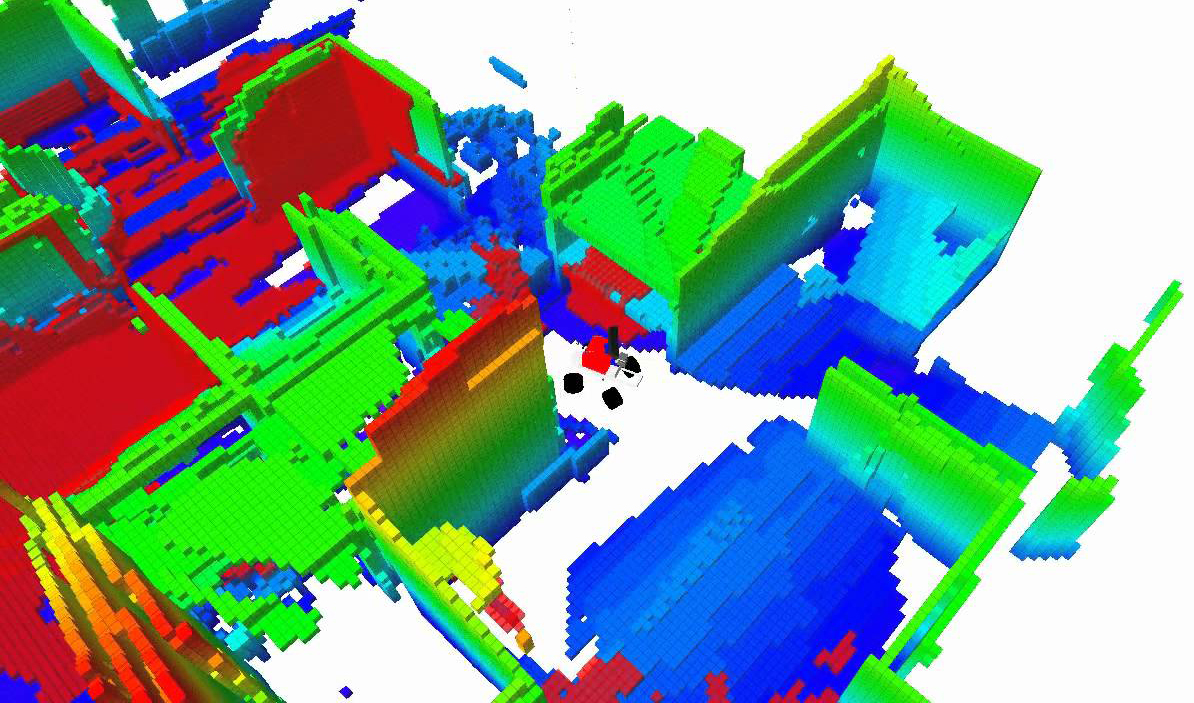
\includegraphics[width=0.7\textwidth, height=0.3\textwidth]{Figures/grid1.jpg}
\caption{Example of a three-dimensional (3D) occupancy grid map. Adapted from~\cite{octomap}.}
\label{fig:occgrid}
\end{center}
\end{figure} 
\textit{Simultaneous localisation and mapping} (SLAM) however, presents solutions that concurrently realises map building and localisation~\cite{slam}. SLAM can be described as utilising both the sensor measurements and control inputs of the robot to construct a continuously expanding map of features in the surrounding environment, while concurrently estimating it's location with respect to these features. The sensor measurements provide information about the robot's environment and the control inputs provide the information about how the robot is moving. A SLAM map typically represents the locations of it's features as a \textit{sparse} set (as opposed to a dense occupancy grid map). An example of a SLAM map is depicted in Figure~\ref{fig:map}. 

The relationship between map building and localisation remains essential to the SLAM problem. If the localisation technique is incorrect, subsequently obtained sensor information will be incorrect, resulting in map estimates that differ from the actual state of the environment. An incorrectly modelled environment will render the sensor information useless, as this information will not correspond with those expected by the constructed map. Ultimately, the resulting localisation approximation will drift over time and eventually become extremely inaccurate. Most modern realisations of SLAM rely on certain probabilistic methods, namely \textit{recursive state estimation} to provide suitable estimates that minimise the uncertainty regarding the mapping and localisation relationship. 

The most commonly used recursive state estimation techniques include both~\textit{optimal filtering} techniques~\cite{ekfslam} as well as \textit{sequential importance sampling} (SIS)~\cite{fast,fast2}. The differences regarding the aforementioned methods can be described as follows: an optimal filtering technique only considers a single hypothesis upon modelling, whereas SIS multiple hypothesis to be considered. A further summary regarding the aforementioned probabilistic approaches is provided in a study by Chen~\cite{chen2003}.

\begin{figure}[H]
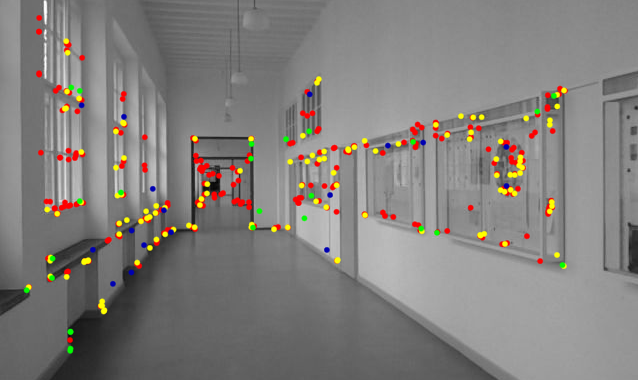
\includegraphics[width=0.49\textwidth, height=0.3\textwidth]{Figures/PTAM_cam.png}
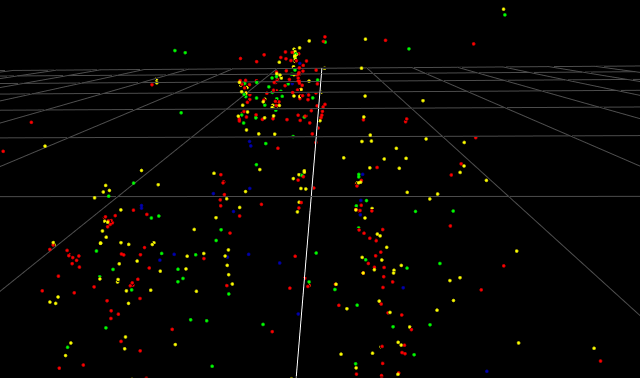
\includegraphics[width=0.49\textwidth, height=0.3\textwidth]{Figures/PTAM_map.png}
\caption{Left: Image frame indicating the feature points. Colours represent the size of a feature (warm colours being the smallest and cool colours being the largest). Right: Reconstructed SLAM three-dimensional (3D) map depicting the feature points with respect to a ground plane (shown as a grid). Adapted from~\cite{scale_visodom}.}
\label{fig:map}
\end{figure}

%Other fundamental parameters and specifications (type of measurement sensor, map dimensionality and sparsity etc.) also determine which specific implementation of the SLAM problem is most applicable. Generally, the main distinguishment between the various realisations of SLAM is the choice of sensor. \\\\
The choice of SLAM implementation will primarily depend on the type of sensor(s) along with the time constraint imposed upon the application (e.g. online map generation vs. offline map generation). Furthermore parameters such as the resultant map's dimensionality as well as their sparsity representation (e.g. point clouds, occupancy grids or sparse sets) are considered upon a suitable SLAM implementation. 

Figure~\ref{fig:slam} depicts the SLAM procedure and is further explained in Table~\ref{tab:Slam}. The robot stores an internal representation (or estimate) of the positions of the features, it's pose as well as the uncertainty associated with each of these entities. It should be noted that these uncertainties are not statistically independent of one another. At each frame, a \textit{prediction} regarding the robot's pose, a \textit{measurement} of the observed feature and an \textit{update} of the internal representation is made. 
%\subsubsection{Range Finder Approaches}
%Range finder approaches utilise a beam or a wave to determine the distance to an obstacle in the environment. Generally, the distance to an obstacle from the range finder can be obtained through measuring the time it takes for a pulse generated in a beam/wave to return to the transmitter, after it has reflected off the obstacle. Two-dimensional range finders are only able to obtain these aforementioned distances in a given plane at an opening angle (e.g. range finders with an opening angle of $180^{\circ}$ obtain all range measurements within a $180^{\circ}$ field of view in the given plane). Three-dimensional range finders however, aren't limited to a single plane and can obtain range measurements in all planes within a field of view equivalent to the opening angle. The 3D point in space where the pulse is reflected can then be reconstructed given that the orientation of the range finder are known, resulting in a 3D point cloud. Range finder approaches include sonar, laser, infra-red and ultrasonic. Laser range finders, more commonly referred to as LIDAR (Light Detection And Ranging) are generally considered to provide the best accuracy, especially with regard to depth measurements. The choice of range finder however, varies dependent on the application and specifications of the system at hand.\\
%Range finders obtain large amounts of data regarding the range to obstacles in the environment, especially in the 3D map case. As a result, non-probabilistic methods (as opposed to those previously discussed) are implemented. One such method, namely \textit{scan matching}, aims to merge overlapping point clouds into a single point cloud. This approach, like many range finder approaches however, generally present a great cost in both processing as well as finance. 

\begin{figure}[H]
\begin{center}
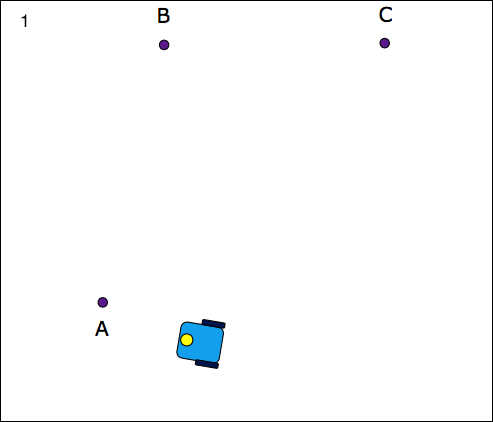
\includegraphics[width=0.32\textwidth, height=0.25\textwidth]{Figures/step1.png}
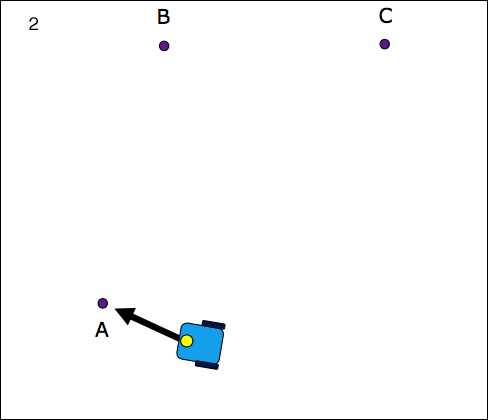
\includegraphics[width=0.32\textwidth, height=0.25\textwidth]{Figures/step2.png}
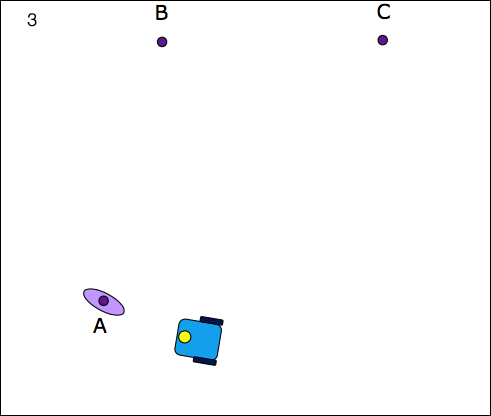
\includegraphics[width=0.32\textwidth, height=0.25\textwidth]{Figures/step3.png}
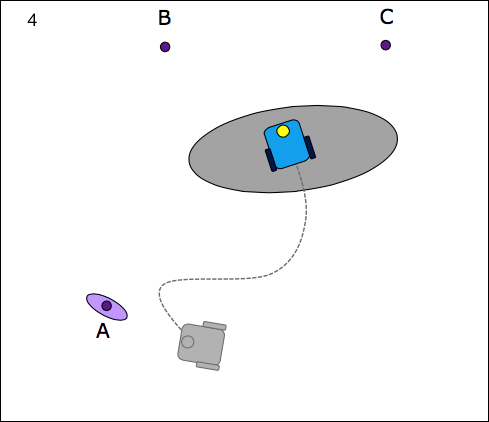
\includegraphics[width=0.32\textwidth, height=0.25\textwidth]{Figures/step4.png}
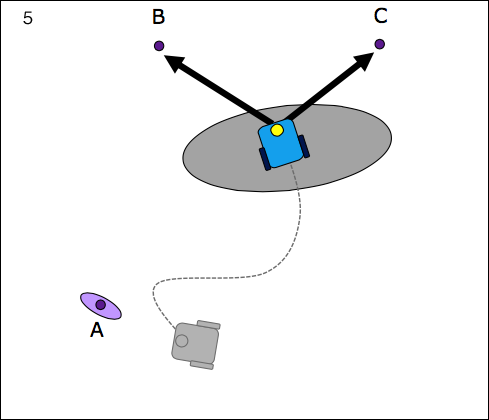
\includegraphics[width=0.32\textwidth, height=0.25\textwidth]{Figures/step5.png}
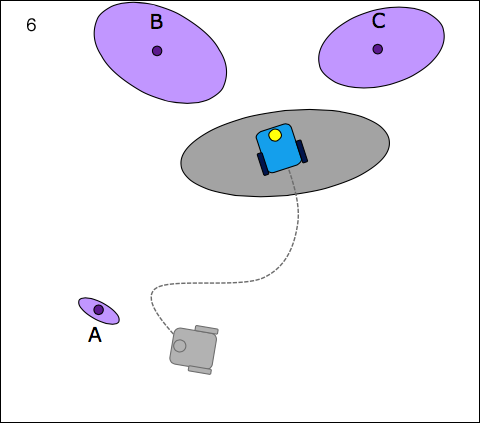
\includegraphics[width=0.32\textwidth, height=0.25\textwidth]{Figures/step6.png}
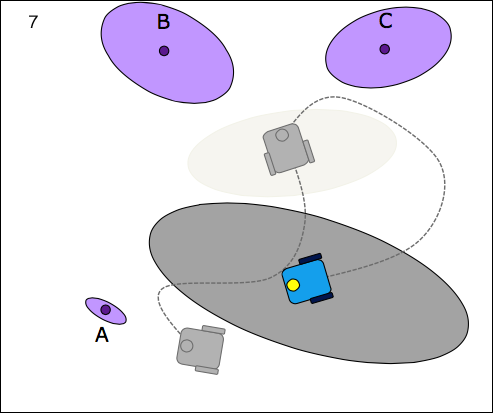
\includegraphics[width=0.32\textwidth, height=0.25\textwidth]{Figures/step7.png}
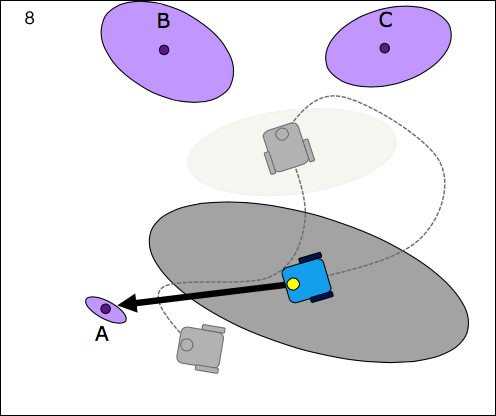
\includegraphics[width=0.32\textwidth, height=0.25\textwidth]{Figures/step8.png}
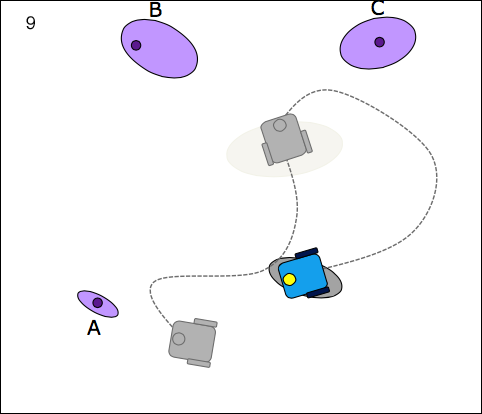
\includegraphics[width=0.32\textwidth, height=0.25\textwidth]{Figures/step9.png}
\caption{A basic representation of the SLAM procedure. Grey ellipses depict uncertainty regarding the robot's pose and purple ellipses depict uncertainty regarding the feature positions. Adapted from~\cite{step1}.}
\label{fig:slam}
\end{center}
\end{figure}

\begin{table}[h]
\caption{SLAM individual steps.}
%\begin{center}
\begin{tabular}{|l|l|}
\hline
Image & \multicolumn{1}{|c|}{Process} \\
\hline
$1-3$ & \pbox{15cm}{Robot begins exploration, observes feature A and updates the internal representation accordingly.}\\
\hline
$4$ & Robot moves, subsequently increasing uncertainty regarding it's pose.\\
\hline
$5-6$ & \pbox{15cm}{Robot observes features B and C and updates the internal representation. Note that the increase in pose uncertainty yields a greater uncertainty in feature position due to the relationship between the robot's pose and the feature estimates.}\\
\hline
$7-8$ & \pbox{15cm}{Robot moves, again increasing uncertainty regarding it's pose before re-observing old feature A. This is referred to as \textit{loop closure}.} \\
\hline
$9$ & \pbox{15cm}{Because the feature locations and robot's pose estimates are not statistically independent, The uncertainty regarding the pose as well as that of all feature positions decreases.}\\
\hline
\end{tabular}
%\end{center}
\label{tab:Slam}
\end{table}% 

\textit{A feature can also be referred to as a landmark and the aforementioned terms will from hereon in be used synonymously.}
%\newpage
%%%%%%%%%%%%%%%%%%%%%%%%%%%%%%%%%%%%%%%%%%%%%%%%%%%%%%%%%%%%%%%%%%%%%%%%%%           
%\subsubsection{Vision Based Approaches}
%Vision based approaches utilise the data captured from cameras. Camera's project the 3D features they observe in the world around them onto a 2D \textit{image plane}. Once projected, the 2D image is then digitised into pixel coordinates where they can then be interpreted, analysed and manipulated in software. There has been a great improvement in the quality of data captured by cameras in the past decade, allowing very reliable projections of the environment. Additionally, cameras are compact, reliable and relatively low-cost with respect to alternative sensors used in SLAM implementations.\\\\
%Camera systems can be configured in different ways to realise SLAM, utilising anything from a single camera to many calibrated cameras. Each configuration yields it's unique advantages (as well as disadvantages) with successful published implementations existing for each configuration. The two most popular implementations include that of a single camera system and that of a stereo pair. Each of the aforementioned implementations are briefly described below along with their respective pros and cons: 
%\begin{enumerate}
%\item \textbf{Single Camera}\\
%Single camera systems (a.k.a monocular systems) rely on using the image data of a single camera only. Although there have been various successful implementations and variations using single camera systems~\cite{dav2007,ptam,visodom}, it remains an issue that the depth of a feature cannot be recovered from a single image. The utilisation of a single camera however, ensures a lower cost as well as a relatively simple SLAM realisation as apposed to that of alternative SLAM approaches.
%\item\textbf{Stereo Calibrated Camera Pair} 
%\\Stereo camera pairs utilise two identical cameras fixed at a given distance between them. These systems are able to effectively recover the depth of a feature in an image from a single observation, through matching a this feature across both images. The setup for such a system however, is somewhat complex as the individual cameras are required to be carefully calibrated. Additionally, stereo systems generally provide a greater computational and financial expense than that of a monocular system.   
%\end{enumerate}
%A meaningful comparison between the aforementioned algorithms is given by~\cite{comp}. 
\newpage
%%%%%%%%%%%%%%%%%%%%%%%%%%%%%%%%%%%%%%%%%%%%%%%%%%%%%%%%%%%%%%%%%%%%%%%%%%    
\subsection{Problem Description}
A vision-based autonomous vehicle operating within an unknown and restricted environment requires a constant update regarding it's \textit{current location}. Many autonomous systems have limited knowledge regarding the surrounding environment but may possess a sensor capable of observing the environment - in this case a camera. It is therefore essential that a solution to this specific localisation problem incorporates the ability to use sensor measurements to build a map on the fly while concurrently locating itself within the map. In a restricted environment, it is likely that a robot will return to a previously observed region, making it essential to incorporate robust \textit{repeatable} localisation where drift from ground truth can be corrected. % Cameras are easily accessible, relatively accurate sensors that are far less expensive than other sensors such as ultrasonic or laser rangefinder sensors. A vision-based solution that utilises a camera should therefore be considered.

Vision-based SLAM implementations as depicted in Figure~\ref{fig:slam} provide the necessary functionality to achieve repeatable localisation. SLAM algorithms utilising single cameras~\cite{dav2007,sola,ptam} have provided elegant yet accurate solutions to the SLAM problem, reconstructing accurate SLAM maps and subsequently, localisation. One such algorithm presented by Davison et al.~\cite{dav2007}, termed MonoSLAM, allows for real-time repeatable localisation of a handheld camera moving within a restricted environment. MonoSLAM, along with the work proceeding it~\cite{dav2007,highspeed2008,scale2010,idp}, has achieved successful results in retrieving the trajectory of a robot, forming a persistent SLAM map and ultimately maintaining repeatable localisation. Although a map of features is not the desired outcome, it remains essential to solving the localisation problem. 

There are however, inherent disadvantages of a MonoSLAM system. Firstly, the utilisation of a single camera prohibits the system from immediately obtaining an accurate depth estimate. A feature is required to be observed from several different viewpoints before an accurate depth estimate can be made. Secondly, the motion model, namely a \textit{constant linear and angular velocity} model, constrains the movement of the system to smooth trajectories - as depicted in Figure~\ref{fig:camvel}. If erratic forces or disturbances act upon the system, the pose of the robot is generally lost, and in most cases irrecoverable. Lastly, because there is no sufficient knowledge of the motion of the robot, the practical applications of the system are vastly limited. 

Information obtained from additional sensors could potentially improve the disadvantages presented by MonoSLAM. Implementations of single camera SLAM using information from an additional measurement sensor (e.g. a laser range finder), such as that presented in a study by Fu et al.~\cite{lasermono}, are not only too expensive but would be difficult to integrate with a single camera system. A more elegant solution that uses measurements to improve the motion estimates is required.   

To extend the range of practical applications of MonoSLAM, a motion model capable of estimating the pose of a robot due to a variety of movements is essential. The current constant linear and angular velocity model limits the robot to smooth movements~\ref{fig:camvel} and therefore needs to be adjusted or replaced. Using additional information can provide the current velocity motion model with better state estimates, but cannot allow movements that aren't ``smooth". Davison et. al~\cite{dav2007}, confirms that additional information such as angular rates obtained from a \textit{gyroscope} improve the state estimates, but cannot compensate for a change in model dynamics. 

A \textit{kinematic estimator} directly measures the derivatives (first and second order) of the position and orientation of the robot as opposed to calculating them from the control inputs and the system's physical model. Inertial measurement units (IMU) can directly measure these derivates and typically comprise of an accelerometer and a gyroscope (and sometimes a magnetometer) that record the accelerations and angular rates respectively. Incorporating such a sub-system could allow a wider variety of practical applications as the physical model of the target system is irrelevant.
\begin{figure}[H]
\begin{center}
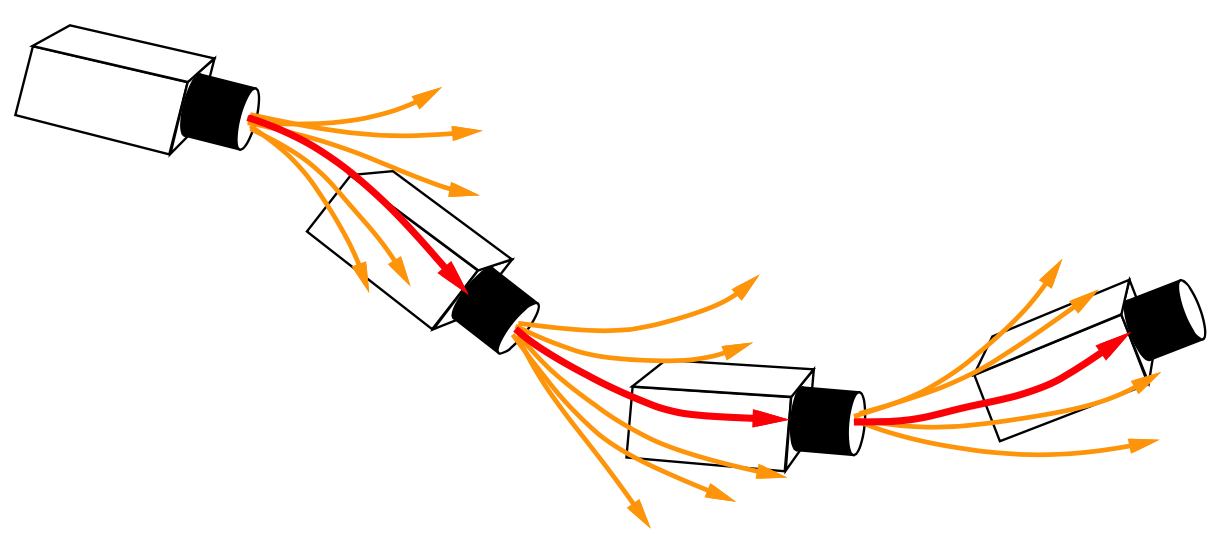
\includegraphics[width=0.48\textwidth, height=0.2\textwidth]{Figures/camvel.png}
\caption{Visualisation of the smooth trajectories of the constant velocity model. Adapted from~\cite{dav2007}}
\label{fig:camvel}
%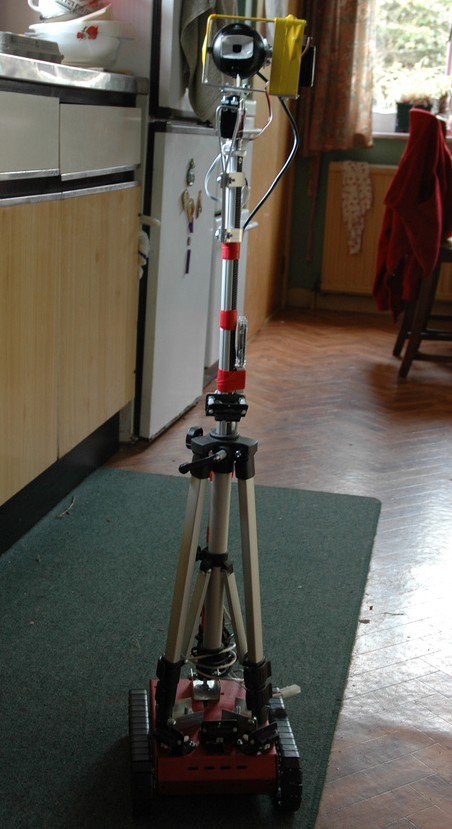
\includegraphics[width=\textwidth, height=0.5\textwidth]{Figures/rob.jpg}
\end{center}
\end{figure}

\subsection{Project Objectives}
This project seeks to utilise the aforementioned MonoSLAM system of Davison et al. and improve the localisation thereof by using \textit{additional} sensor information. The improvement(s) of the system should allow the existing system to obtain better localisation and extend the range of applications upon which the system can be applied while maintaining the original performance standard: repeatable localisation at 30 Hz for approximately 100 features. The system should utilise a \textit{single} camera as the measurement sensor and preferably support real-time operation. All processing regarding the SLAM algorithm can be done on a standard PC that communicates with sensors via a serial port. The project budget is R $1500.00$. 
\\\\
The primary objectives of this study include:
\begin{itemize}
\item \textbf{Performing an overview on the current techniques used to realise SLAM} \\
In order to understand how SLAM is implemented, an understanding of probability theory and state estimation is required. These concepts - specifically recursive state estimation and the Bayes Filter - need to be researched and analysed before choosing a suitable technique to implement.
\item \textbf{Analysis of the kinematic estimator as an alternative motion model}\\
A kinematic estimator is suggested as a alternative motion model. The kinematic estimator needs to be researched, mathematically derived and simulated. The results from the simulation should correspond to the mathematical derivation. The advantages and disadvantages of the kinematic estimator also need to be investigated.
\item \textbf{Hardware Design of the System} \\
The kinematic estimator requires additional measurements obtained from an IMU. The IMU is required to interface with the PC via a micro-controller. The micro-controller allows precise synchronisation between the images sampled by the camera and the IMU measurements. A functional diagram of the system's hardware components are depicted in Figure~\ref{fig:sys}. 
\item \textbf{Comparison between proposed and original MonoSLAM implementations}\\
If time allows, a set of tests are required to be derived and implemented to establish whether the proposed improvement(s) actually adhere to the problem description.  
\end{itemize}
\begin{figure}[h]
%\begin{center}
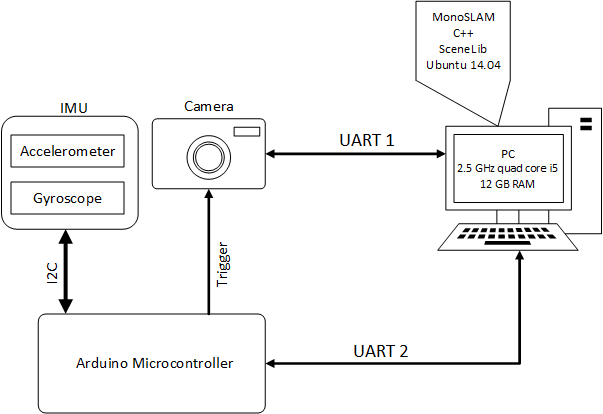
\includegraphics[width=\textwidth, height=0.6\textwidth]{Figures/Drawing2.png}
\caption{Functional diagram of the interaction between the system's hardware components}
\label{fig:sys}
%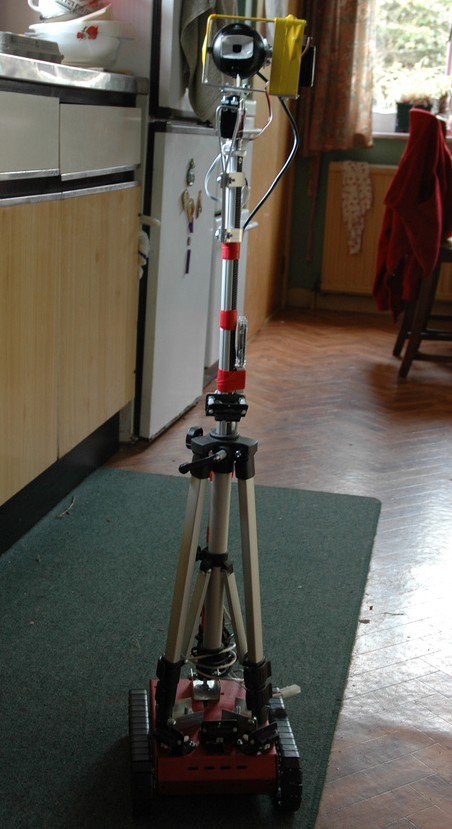
\includegraphics[width=\textwidth, height=0.5\textwidth]{Figures/rob.jpg}
%\end{center}
\end{figure}

%It is initially assumed that these measurements provide the necessary information to improve motion estimates. This project will primarily focus on deriving an accurate kinematic estimator as the motion model of a MonoSLAM system that incorporates inertial measurements to better approximate the trajectory of a robot. 
%An EKF (EKF) is chosen as the probabilistic method that realises the solution to the SLAM problem. The EKF is chosen for its simplicity to implement and because it is assumed that the Unscented KF (UKF)\textcolor{red}{[ref]} will only provide a greater efficiency if the number of landmarks are large. Considering that a restricted environment is being explored by the robot, it is expected as presented by Davison et al.~\cite{dav2007}, that the number of landmarks present in the SLAM map will not exceed 100. Furthermore it is assumed that a first order linearisation presents a good enough approximation for the modelling of the system dynamics. 

%The process regarding the construction of this map of features, namely that of recursive state estimation, is to be implemented through the use of an (Extended) KF. The map initially, completely void of any landmarks, is recursively updated according to the subsequent fusions of both the prediction and  the measurement presented to the KF. As new (potentially interesting) features are observed, the state estimates of both the camera as well as the landmarks are both updated - augmenting the state vector with additional features (if indeed they are observed) while deleting any landmarks that are no longer of interest. In order to obtain the best possible result, the algorithm should strive to obtain accurate state estimation regarding the movement of the robot as well as a sparse set of high-quality landmarks. Each of the steps regarding the realisation of the previously mentioned map of features are to be defined, described and analysed in the sections that follow. 
%The ultimate goal of any three dimensional (3D) SLAM approach, is to obtain a probabilistic 3D map of point features, representing at every time instance, the estimates of both the state of the robot as well as the positions of every feature observed. The previously mentioned features of interest are more commonly referred to as \textit{landmarks} and the aforementioned terms will, from hereon in, be used synonymously.  Most importantly though, the map is to contain the \textit{uncertainty} associated with each of the aforementioned estimates.\\ The past decade however, has yielded many acceptable and impressive solutions as in~\cite{highspeed2008, scale2010,srukf}, to the aforementioned requirements using a single camera, with the original proposal presented by Davison et al.~\cite{dav2007}, more commonly referred to as MonoSLAM (Monocular vision based SLAM). In MonoSLAM, the robot is set to \textbf{only} obtain sensor information through the utilisation of a singular camera system. There are however, inherent disadvantages of such a system: Firstly, the utilisation of a single camera prevents the system from immediately obtaining an accurate depth estimate. Landmarks are required to be examined from various viewpoints before an appropriate depth estimation can be concluded. Secondly, the motion model (namely a constant velocity model) constrains the movement of the system to smooth, constant trajectories. In the event that erratic, immediate disturbances act upon the system, the pose of the robot is generally lost, and in most cases irrecoverable. Lastly, because no sufficient knowledge regarding the movement of the robot exists - its practical application is vastly limited. \\The proposed approach to be presented in the following paper, aims to improve the system to limit of these disadvantages, namely the latter two. This paper aims to extend the aforementioned system of Davison with the utilisation of \textit{additional} sensor information regarding the robot's motion. An inertial measurement unit (IMU) will provide this additional information, recording the movement of the robot through space as a result of the control inputs to the system. The additional data allows the system to be modelled as a rigid, kinematic body upon which kinematic estimation can be applied. Inevitably, a kinematic estimator allows the system a greater knowledge of its movement - because it is being measured through inertial sensors.\\\\
%The process regarding the construction of this map of features, namely that of recursive state estimation, is to be implemented through the use of an (Extended) KF. The map initially, completely void of any landmarks, is recursively updated according to the subsequent fusions of both the prediction and  the measurement presented to the KF. As new (potentially interesting) features are observed, the state estimates of both the camera as well as the landmarks are both updated - augmenting the state vector with additional features (if indeed they are observed) while deleting any landmarks that are no longer of interest. In order to obtain the best possible result, the algorithm should strive to obtain accurate state estimation regarding the movement of the robot as well as a sparse set of high-quality landmarks. Each of the steps regarding the realisation of the previously mentioned map of features are to be defined, described and analysed in the sections that follow. 
%\newpage
%The intended contribution of this paper realises an improvement in not only the state estimation of the system, but localisation as a whole. Additionally the kinematic estimator embedded within the system should serve as a means to integrate the proposed system as part of a larger system regardless of that system's physical model.  Moreover, the proposed system is required to operate in real time at a rate of at least the 30 Hz for 100 landmarks; as achieved by Davison in his original work presented in \cite{dav2007}.  
%%%%%%%%%%%%%%%%%%%%%%%%%%%%%%%%%%%%%%%%%%%%%%%%%%%%%%%%%%%%%%%%%%%%%%%%%%
\subsection{Project Outline}
The remainder of this report is presented as follows:\\\\
\textbf{Chapter 2: Probabilistic State Estimation Techniques}\\
This chapter presents all of the research undertaken in order to effectively design and implement a suitable SLAM implementation. This chapter focusses of introducing the reader to the basic theory pertaining to probability theory and recursive state estimation and presenting the relevant mathematical expressions that model them. The chapter further introduces the steps necessary to derive the EKF from the Bayes Filter. \\\\
\textbf{Chapter 3: System Design}\\
This chapter provides a detailed overview of the solution to the MonoSLAM problem. The relevant variable representation and functional components are initially discussed. The chapter then seeks to derive the kinematic estimator necessary for the EKF's prediction step. An overview of the EKF's measurement update is also given.\\\\
\textbf{Chapter 4: Implementation}\\
This chapter sets out to predict the behaviour of the various sub-systems through simulation. The results from the analysis of the kinematic estimator, EKF and IMU are all analysed accordingly.\\\\
\textbf{Chapter 5: Testing and Results}\\
This chapter presents all the relevant tests carried out to determine the proposals validity. The results of these tests are subsequently analysed.\\\\
\textbf{Chapter 6: Conclusions and Recommendations}\\
This chapter provides a summary recommendations by the author that is applicable to future work. The final conclusion is formulated analysing the state of the final system compared to the objectives of the project. 
\newpage
%%%%%%%%%%%%%%%%%%%%%%%%%%%%%%%%%%%%%%%%%%%%%%%%%%%%%%%%%%%%%%%%%%%%%%%%%%    
%\section{Literature Study}
%\newpage
%%%%%%%%%%%%%%%%%%%%%%%%%%%%%%%%%%%%%%%%%%%%%%%%%%%%%%%%%%%%%%%%%%%%%%%%%%    
\section{Theory: Probabilistic State Estimation Techniques}
\subsection{Introduction}
The following chapter will provide a brief, yet concise introduction to the fundamental algorithms that are necessary to implement SLAM. The fundamental concepts, particularly the various techniques associated with the implementation thereof will be addressed. The goal of this section is to introduce the fundamental concepts as well as the mathematical and probabilistic principles that form the basis of state estimation in the robotics field of study.

Initially, the Bayes Filter; that is the algorithm that forms the basis of all state estimation techniques presented in this report, will be introduced and formally discussed. Thereafter, the Gaussian Filter family - particularly the \textit{Kalman Filter} (KF) as well as it's variants - are to be introduced, discussed and defined in terms of the context of this project. It is worthwhile to note that theory in this chapter resembles material from the book Probabilistic Robotics by Thrun et al.~\cite{probrob} and is adapted therefrom for convenience sake.  
%This chapter provides a brief, yet concise introduction to the fundamental theoretical concepts and algorithms that are necessary to implement SLAM. Firstly, the concept of estimating state variables using a motion model and sensor measurements is initially described. The chapter then presents a suitable state estimation method, namely the Bayes filter. Additionally, the KF, a particular implementation of the Bayes filter is derived. Finally, the KF is appropriately extended to present the EKF, the state estimation algorithm chosen to realise this project.    

\subsection{Recursive State Estimation}
 %Quantities exist that are not directly observable, yet are still able to be obtained through sensor data. Sensors though, obtain limited data regarding certain quantities and most importantly, are affected and often corrupted by \textit{noise}.   
%Probabilistic robotics yields a unique yet fundamental concept at its core, that is: estimating a state through sensor data. \\
State variables define the mathematical state of a system's dynamics and describe the impact of the system's future behaviour in the absence of external factors. Although a robot's dynamics can be mathematically modelled, they have quantities that are not directly observable but can be obtained through sensor measurements. Sensors though, obtain limited data regarding certain quantities and most importantly, are affected and often corrupted by \textit{noise}.

State estimation then, seeks to recover state variables using obtained sensor data, control inputs to the system as well as the system model. The value obtained is referred to as a \textit{state estimate}. In the case of SLAM, the state estimates of a robot incorporate the robot's pose as well the position of each landmark in the environment.  

\textit{Recursive state estimation} however, doesn't require the system to keep a complete history of \textit{all} measurements and control inputs, using only the current control inputs and measurements to update the previous state estimate. Probabilistic state estimation algorithms - to be investigated in this section - compute \textit{belief} distributions regarding state variables where the belief reflects a robot's internal knowledge of it's state. 

In the case of SLAM, the robot is required to know its location at each time instance $t$. The belief must thus be calculated at each time step.  In order to achieve recursive state estimation, the state estimates of the robot should only incorporate the latest measurements. Additionally, the calculation of the belief should incorporate the previous estimates. Provided that the the system also obeys the Markov assumption - previous data and future data are independent provided that the current state $\textbf{x}_t$ is known - the \textit{Bayes Filter} provides such recursive state estimation. 
\newpage
%%%%%%%%%%%%%%%%%%%%%%%%%%%%%%%%%%%%%%%%%%%%%%%%%%%%%%%%%%%%%%%%%%%%%%%%%%
\subsection{Bayes Filter}
The previously mentioned belief of a robot can be represented by a probability distribution that assigns a probability to each state outcome. The belief distribution is a posterior probability over the state variable that is conditioned over the measurements and control data~\cite{probrob}. Mathematically the belief with regard to a state variable $\textbf{x}_t$ is as shown in the book Probabilistic Robotics by Thrun et al.~\cite{probrob}:     
%A key concept worth describing is the previously mentioned \textit{belief} of a robot. The belief represents the robot's understanding regarding the state of it's own dynamics (it's position, orientation etc.) as well as that of the surrounding environment. This critical concept proves a fundamental basis in probabilistic robotics. The belief can be represented as a conditional probability distribution whereby each possible scenario (state) is assigned a probability (density). 
\begin{equation} \label{eq:belief}
bel(\textbf{x}_t) = p(\textbf{x}_t\hspace{0.1cm}|\hspace{0.1cm}\textbf{z}_{1,..,t},\hspace{0.1cm}\textbf{u}_{1,..,t}).
\end{equation}

This describes, for a given time $t$, a joint density of the robot state as well as the landmark locations {given} all of the previously recorded observations ${z}_{1:t}$ and control inputs ${u}_{1:t}$.
%Considering that the state of the robot is constantly updated at every time-step $t$ and that each update is dependent upon the state at the previous time-step, it is essential that the algorithm required be recursive in nature. The \textit{Bayes Filter} algorithm provides precisely such a procedure. The algorithm calculates the belief distribution stated in equation~\ref{eq:belief} from the observation and control data. 
Table~\ref{tab:KF} presents a pseudo-algorithm of the Bayes Filter algorithm \cite{probrob}:

\begin{table}[h]
\begin{center}
\caption{The Bayes Filter Algorithm} \label{tab:BF}
\begin{tabular}{l l l}
\hline
\textbf{Input}: &previous belief $bel(\textbf{x}_{t-1})$, control input(s) $\textbf{u}_t$, measurement(s) $\textbf{z}_t$\\ 
\textbf{Output}: &current belief $bel(\textbf{x}_{t})$\\
\hline
\hline
for all $\textbf{x}_t$: \\
1. & $\overline {bel}(\textbf{x}_t)$ = $\int p(\textbf{x}_t\hspace{0.1cm}|\hspace{0.1cm}\textbf{u}_{t},\hspace{0.1cm}\textbf{x}_{t-1})bel(\textbf{x}_{t-1})d\textbf{x}_{t-1}$ \\
2. & ${bel}(\textbf{x}_t)$ = $\eta p(\textbf{z}_t\hspace{0.1cm}|\hspace{0.1cm}\textbf{x}_{t})\overline {bel}(\textbf{x}_t)$ \\
3. &end for. \\
\hline\hline
\end{tabular}
\end{center}
\end{table}%
The recursive nature of the algorithm can thus be seen from Table~\ref{tab:BF}; whereby the belief $\overline {bel}(\textbf{x}_t)$ at the current time $t$ is obtained through initially calculating the belief at the previous time-step, $t-1$. The Bayes Filter contains two essential steps: \textit{prediction} (line 1) and \textit{measurement update} (line 2). The prediction step initially processes the control inputs before subsequently predicting the current belief based on the prior belief and the probability that a transition from $\textbf{x}_{t-1}$ to $\textbf{x}_t$ occurs. Thereafter, the measurement update improves the belief by adding information about the states, observed from new measurements.

The Bayes Filter can be implemented in many different ways. Upon choosing a suitable implementation, a trade off between the following properties needs to be made:
\begin{itemize}
\item Computational efficiency
\item Accuracy of the approximation 
\item Ease of Implementation
\end{itemize}
   
The mathematical derivation of the Bayes Filter contains many assumptions and further technicalities. The techniques presented in this project require only a basic understanding of the Bayes Filter. A detailed analysis of the Bayes Filter can be obtained from the book Probabilistic Robotics by Thrun et al.~\cite{probrob}. 
%%%%%%%%%%%%%%%%%%%%%%%%%%%%%%%%%%%%%%%%%%%%%%%%%%%%%%%%%%%%%%%%%%%%%%%%%%
\newpage
\subsection{Gaussian Filters}
%%%%%%%%%%%%%%%%%%%%%%%%%%%%%%%%%%%%%%%%%%%%%%%%%%%%%%%%%%%%%%%%%%%%%%%%%%
Amongst the many different implementations of the Bayes Filter are the \textit{Gaussian filter} family. The basic idea behind a Gaussian filter is that beliefs can be represented as a multivariate Gaussian distributions, represented mathematically as follows~\cite{probrob}:
\begin{equation} \label{eq:normal}
p(\textbf{x}_t)=\cfrac{1}{\sqrt{|2\pi\boldsymbol{\Sigma}|}}\hspace{0.1cm}\text{exp}\hspace{0.1cm}\bigg\{-\frac{1}{2}(\textbf{x}_t-\boldsymbol{\mu})^T\boldsymbol{\Sigma}^{-1}(\textbf{x}_t-\boldsymbol{\mu})\bigg\},
\end{equation} 
where the density across the state variable $\textbf{x}_t$ is characterised through two fundamental parameters: the mean $\boldsymbol{\mu}$ and the covariance $\boldsymbol{\Sigma}$. Such a parameterisation whereby a Gaussian is characterised through it's respective mean and covariance is called the \textit{moments parameterisation} (as the mean and covariance represent the first and second order moments respectively). AThis parameterisation allows a number of recursive filter algorithms to be derived, two of which are examined in this project: the \textit{KF} (KF) and it's non-linear counterpart, the \textit{EKF} (EKF). It is important to realise that both of the aforementioned filters belong to the same sub-class of filters - namely the KF Family - and therefore most of the fundamental concepts and functionality between them are identical. Each filter is discussed in further detail in the subsections that follow.   
%%%%%%%%%%%%%%%%%%%%%%%%%%%%%%%%%%%%%%%%%%%%%%%%%%%%%%%%%%%%%%%%%%%%%%%%%%
\subsubsection{KF}    
Probably the most fundamental of all Gaussian filter algorithms, is the \textit{KF}. The KF can be briefly described as an optimal estimator. It remains a popular technique for filtering and prediction of \textit{linear} systems that contains Gaussian uncertainty. The KF seeks to describe a belief distribution of a state variable $\textbf{{x}}_t$ as described in Equation~\ref{eq:normal}. Subsequently, the state vector $\textbf{{x}}_t$ is modelled by a single multivariate Gaussian distribution with a mean $\boldsymbol{\mu}_t$ and covariance $\boldsymbol{\Sigma}_t$, at each time instance $t$ (while previous time-steps are denoted as $t-1$, $t-2$, etc.). The general implementation as described above though, is only valid provided that the following three properties hold true - as listed in~\cite{probrob}: 
\begin{enumerate}
\item The state transition model probability \textbf{must} be a \textit{linear} function with additive Gaussian (process) noise. The state transition model probability is shown according to Thrun et al.\cite{probrob}:\\
\begin{equation}\label{eq:SSmodelg}
g(\textbf{u}_{t}, \textbf{x}_{t-1}) :  \textbf{x}_t = \textbf{A}_t\textbf{x}_{t-1} + \textbf{B}_t\textbf{x}_t + \textbf{w}_t.
\end{equation}
\item The observation model probability \textbf{must} be a \textit{linear} function with additive Gaussian (sensor) noise. The observation model probability is shown according to Thrun et al.\cite{probrob}:\\
\begin{equation}\label{eq:SSmodelh}
h(\overline{\boldsymbol{\mu}}_t) : \textbf{z}_t = \textbf{C}_t\textbf{x}_t + \textbf{v}_t,
\end{equation}
where $\textbf{w}_t$ and $\textbf{v}_t$ represent process and sensor noise respectively.
\item The initial belief $bel(\textbf{x}_0)$ must be normally distributed.
\end{enumerate}
%In the context of Simultaneous Localisation and Mapping (SLAM), a KF algorithm seeks to determine the \textbf{optimal} trade off between the state of the robots pose and the position of the landmarks within the map - given process and measurement noise.\\
%provided that the state vector $\textbf{\^{x}}_k$, and landmark locations $\textbf{\^{y}}_{n,k}$ are modelled by a single multivariate Gaussian distribution. The system is to be observed at discrete steps in time - denoted by the subscript$k =1, 2,  3, ...$ - where at every individual time-step, it can be influenced by a set of actions. It is assumed that\\  

%Moreover, the solution to this specific implementation of the SLAM problem, takes a probabilistic form where the belief with regard to state variable $\textbf{x}_t$ is denoted as shown in equation~\ref{eq:belief}:
%\begin{equation}
%bel(\textbf{{x}}_t) = p\big(\textbf{{x}}_t\hspace{0.15cm}|\hspace{0.15cm}\textbf{z}_{1:t},\textbf{u}_{1:t}\big),
%\end{equation}

%with the aforementioned distribution described at every discrete time instance $t$.\\ A brief description would yield that the distribution above, describes, for a given time instance $t$, a joint density of the robot state as well as the landmark locations \textbf{given} all of the previously recorded observations, $\textbf{z}_{1:t}$ and control inputs, $\textbf{u}_{1:t}$.\\

The input to the KF is the belief at time $t-1$, represented by $\boldsymbol{\mu}_{t-1}$ and $\boldsymbol{\Sigma}_{t-1}$. The KF requires a control input $\textbf{u}_t$ and a measurement $\textbf{z}_t$ at time $t$ to update the belief. Like the Bayes Filter, the KF too is executed in two (sequential) steps: the \textit{prediction step} and the \textit{update step}. 

Firstly at time $t$, the prediction step aims to calculate a predicted belief $\overline{bel}(\textbf{x}_t)$ represented by $\overline{\boldsymbol{\mu}_{t}}$ and $\overline{\boldsymbol{\Sigma}_{t}}$. The predicted belief is obtained by incorporating the control input $\textbf{u}_t$ and subsequently updating the mean vector and covariance matrix according to the (linear) state transition function. The update step aims to obtain the desired belief $bel(\textbf{x}_t)$ from the predicted belief $\overline{bel}(\textbf{x}_t)$ by incorporating the measurements $\textbf{z}_t$. The KF computes a Kalman gain, that intuitively suggests the influence of a measurement in the new state estimate. This gain is then used to update the mean estimate as well as the covariance matrix. 

Each of the aforementioned steps are later discussed in more detail - with reference to implementations specific to this paper. Table~\ref{tab:KF} below, presents a pseudo-algorithm of the KF~\cite{probrob}:
% estimate the state into which the system will be transitioned from the previous state estimate ($\boldsymbol{\mu}_{t-1}$, $\boldsymbol{\Sigma}_{t-1}$) as a result of a set of internal and/or external dynamics to the system. These dynamics are typically described through the state transition function $g(\textbf{u}_t, \boldsymbol{\mu}_{t-1})$. Once an estimate is obtained for the transitioned state estimate ($\boldsymbol{\bar \mu}_t$, $\boldsymbol{\bar \Sigma}_t$), a measurement prediction is made in order to provide the expected measurements provided that the system were to find itself within the estimated transitioned state. These measurements are obtained through an observation model which has a function $h(\boldsymbol{\bar \mu}_t)$. Thereafter, an actual measurement, $\textbf{z}_t$ is then obtained through the system sensors in order to determine the actual state of the system ($\boldsymbol{\mu}_t$, $\boldsymbol{\Sigma}_t$). Ultimately, the actual state of the system and the previously predicted state are then compared with one another in order  to obtain the (optimally weighted) \textit{Kalman gain}: This 

\begin{table}[h]
\begin{center}
\caption{The KF Algorithm}\label{tab:KF}
\begin{tabular}{l l l}
\hline
\textbf{Input}: &previous mean $\boldsymbol{\mu}_{t-1}$ and covariance $\boldsymbol{\Sigma}_{t-1}$, control inputs $\textbf{u}_t$, measurements $\textbf{z}_t$\\ 
\textbf{Output}: &mean $\boldsymbol{\mu}_{t}$, covariance $\boldsymbol{\Sigma}_{t}$\\
\hline
\hline
&\textbf{Prediction step} \\
\hline
1. & $\boldsymbol{\bar \mu}_{t}$ = $g(\textbf{u}_{t}, \boldsymbol{\mu}_{t-1})$ = $\textbf{A}_t\hspace{0.05cm}\boldsymbol{\mu}_{t-1} + \textbf{B}_t\hspace{0.05cm}\boldsymbol{\mu}_t$ + $\textbf{w}_t$\\
2. & $\boldsymbol{\bar \Sigma}_t = \textbf{A}_t \boldsymbol{\Sigma}_{t-1} \textbf{A}_t^T + \textbf{R}_{w,t}$ \\
\hline
&\textbf{Correction step}\\
\hline
3. & $\textbf{K}_t = \boldsymbol{\bar \Sigma}_{t} \textbf{C}_t^T (\textbf{C}_t \boldsymbol{\bar \Sigma}_{t} \textbf{C}_t^T + \textbf{R}_{v,t})^{-1}$ \\
4. & $\boldsymbol{\mu}_t = \boldsymbol{\bar \mu}_t + \textbf{K}_t[\textbf{z}_t-\textbf{C}_t\boldsymbol{\bar \mu}_t]$\\  
5. & $\boldsymbol{\Sigma}_{t} = (\textbf{I}-\textbf{K}_t \textbf{C}_t)\boldsymbol{\bar \Sigma}_t$ \\
\hline\hline
\end{tabular}
\end{center}
\end{table}%

The KF is generally considered an efficient algorithm for sparse sets. The \textit{computational complexity} of a matrix inversion is bounded by an order of $O(d^{2.4})$~\cite{probrob}, where d represents the dimensions of the measurements vectro $\textbf{z}_t$.  
%%%%%%%%%%%%%%%%%%%%%%%%%%%%%%%%%%%%%%%%%%%%%%%%%%%%%%%%%%%%%%%%%%%%%%%%%%
\newpage
\subsubsection{EKF} \label{sec:EKF}
Considering that most practical systems of interest yield non-linear behaviour, the KF in its purest form cannot be successfully implemented upon the vast majority of modern day systems. Non-linear transformations of Gaussian random variables (RV) result in a different RV while any linear transformation of a Gaussian random variable yields another \textbf{different} Gaussian variable. This violates an important condition of the KF algorithm. This phenomenon can be illustrated through Figure~\ref{fig:lin}: % where a linear transform yields a transformed Gaussian RV and a non linear transform yields a RV with a different probability density:

\begin{figure}[h]
%\begin{center}
\includegraphics[width=0.49\textwidth, height=0.7\textwidth]{Figures/LIN1.png}
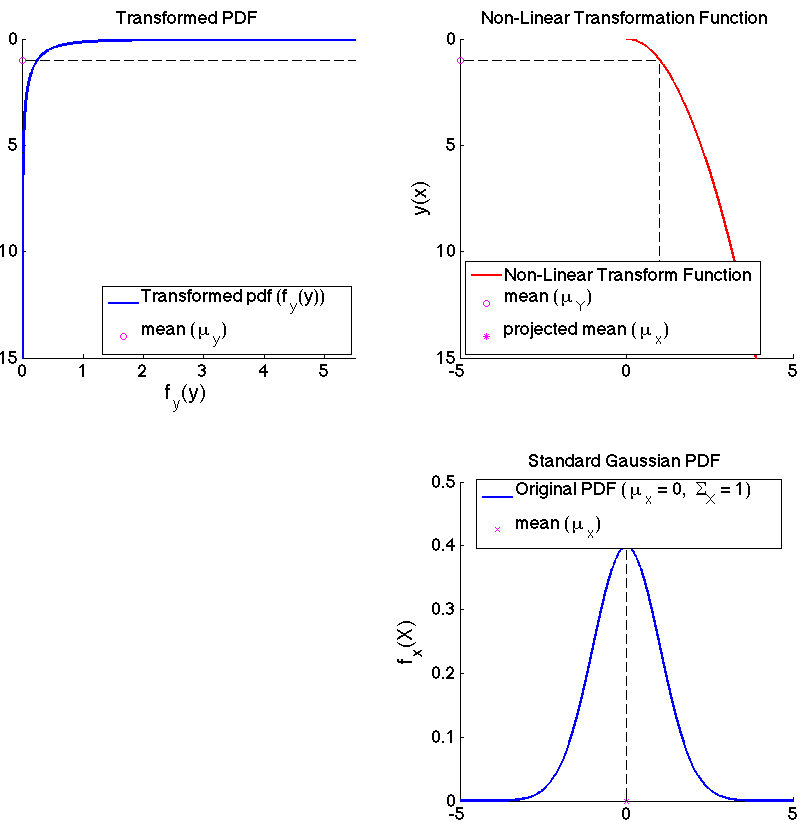
\includegraphics[width=0.49\textwidth, height=0.7\textwidth]{Figures/Non1.png}
\caption{Left: Linear transformation of a Gaussian random variable. Right: Non-linear transformation of a Gaussian random variable.}
\label{fig:lin}
%\end{center}
\end{figure}
%\begin{figure}[h]
%\begin{center}
%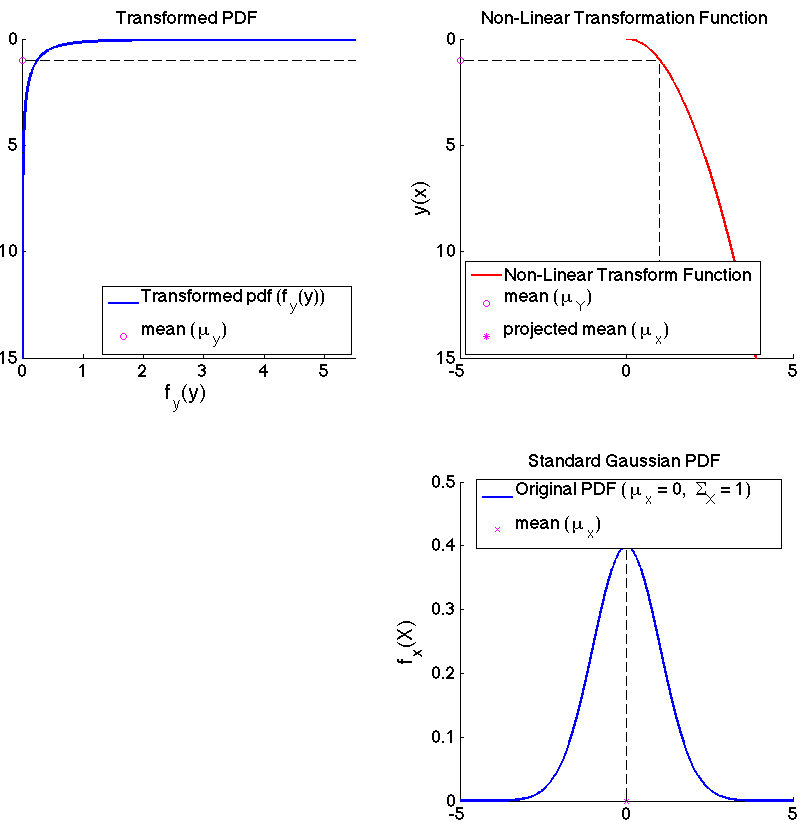
\includegraphics[width=0.49\textwidth, height=0.6\textwidth]{Figures/Non1.png}
%\caption{ Non-linear transformation of a Gaussian random variable.}
%\label{fig:non}
%\end{center}
%\end{figure}
The \textit{EKF} (EKF), an extension of the general KF, aims to enable the modelling of non-linear systems through linearisation. As previously mentioned, the state transition function $g(\textbf{u}_t, \textbf{x}_{t-1})$, as well as the observation model $h(\textbf{x}_{t-1})$ of most practical systems are typically both non-linear in nature. Considering the aforementioned statement; it is necessary to determine a method for approximating a non-linear function as a linear function, more commonly referred to as linearisation. The linearisation process of EKF aims to linearise these functions so that the fundamental operations of the KF algorithm remain valid.

The linearisation process approximates an arbitrary non-linear function $f$ by a linear function that is \textit{tangent} to $f$ at the mean value of the Gaussian, $\boldsymbol{\mu}$. If the Gaussian is then projected through this new linear approximation, the resultant transformation would yield a random variable that is Gaussian in nature (as in Figure~\ref{fig:lin}). This technique is applied to both the state transition and observation functions. Many methods exist for linearisation of non-linear functions, but the EKF utilises the method of (first order) \textit{Taylor expansion}. The Taylor expansion creates a linear approximation of a non linear function, say $f$, by it's own value as well as that of it's gradient $f'$. The tangent of $f$ can be depicted by it's partial derivative with respect to the state vector $\textbf{x}_{t-1}$:
\begin{equation}\label{eq:par}
f'(\textbf{x}_{t-1}, \textbf{u}_t) := \frac{\partial f(\textbf{x}_{t-1}, \textbf{u}_t)}{\partial \textbf{x}_{t-1}}.
\end{equation}

The argument of the function $f$ is chosen as the most likely point at the linearisation instance. For Gaussians, the most likely point is the mean $\mu_{t-1}$. The linear approximation of the function $f$ can then be achieved through the linear extrapolation evaluated at it's most likely point $\mu_{t-1}$:
\begin{equation}\label{eq:app}
\begin{split}
f(\textbf{x}_{t-1}, \textbf{u}_t) &\approx f(\textbf{x}_{t-1}, \textbf{u}_t) + f'(\textbf{u}_{t},\boldsymbol{\mu}_{t-1})(\textbf{x}_{t-1}-\boldsymbol{\mu}_{t-1}) \\
&= f(\textbf{x}_{t-1}, \textbf{u}_t) + \textbf{F}_t'(\textbf{x}_{t-1}-\boldsymbol{\mu}_{t-1}),
\end{split}
\end{equation}
where $\textbf{F}_t' = f'(\textbf{u}_{t},\textbf{x}_{t-1})$ is the \textit{Jacobian} matrix. 

It is important to note that {Jacobian} matrix is determined at each linearisation instance (each individual time-step) as its parameters differ from one linearisation instance to the next. 

%Once linearisation is achieved, the EKF which behaves otherwise identically in terms of operation to the general KF, can be implemented upon non-linear systems. 
It is very important to note that because only a first order Taylor expansion is used to \textit{approximate} the linearisation, severe non-linearities will prohibit acceptable approximations of the Gaussian distribution upon transformations. If the linearisation point is chosen at a point close to the mean, the EKF will yield an acceptable approximation from the linearisation process. 

There are other variants of the KF that aren't discussed in this project, but have been carefully considered. It is assumed that the first order Taylor approximation provides a suitable approximation of the non-linearities that are expected in the system, namely the uncertainty regarding angle orientation errors. The \textit{Unscented KF} is assumed to be a less appropriate choice of filter to the EKF considering the the lack of severe system non-linearities. The objective of the project seeks to provide localisation for a set of approximately 100 landmarks. The \textit{Information Filter} will only provide a better computational complexity than the EKF if the number of landmarks are much larger. This analysis suggests that the EKF provides a suitable yet simple implementation of the Bayes Filter.%The EKF is chosen as a suitable implementation of the Bayes Filter as the non-linearities the first order Taylor approximation is poor due to severe non-linearities. This project however, assumes that the the number of landmarks aren't large enough for the UKF to provide a better efficiency and that the transition and measurement probabilities are reasonably approximated by the Taylor expansion. 

Table~\ref{tab:EKF}  below, systematically and mathematically represents the steps associated with the EKF~\cite{probrob}:

\begin{table}[h]
%\begin{center}
\caption{The EKF Algorithm}\label{tab:EKF}
\begin{tabular}{l l l}
\hline
\textbf{Input}: &previous mean $\boldsymbol{\mu}_{t-1}$ and covariance $\boldsymbol{\Sigma}_{t-1}$, control inputs $\textbf{u}_t$, measurements $\textbf{z}_t$\\ 
\textbf{Output}: &mean $\boldsymbol{\mu}_{t}$, covariance $\boldsymbol{\Sigma}_{t}$\\
\hline
\hline
&\textbf{Prediction step} \\
\hline
1. & $ \boldsymbol{\bar \mu}_t$ = $g(\textbf{u}_t,  \boldsymbol{\bar \mu}_{t-1})$ \\
2. & $\boldsymbol{\bar \Sigma_t} = \textbf{G}_t' \boldsymbol{\bar \Sigma_{t-1}} \textbf{G}_t'^T + \textbf{R}_{w,t}$ \\
\hline
&\textbf{Correction step}\\ 
\hline
3. & $\textbf{K}_t = \boldsymbol{\bar \Sigma_{t}} \textbf{H}_t'^T (\textbf{H}_t' \boldsymbol{\bar \Sigma_{t}} \textbf{H}_t'^T + \textbf{R}_{v,t})^{-1}$ \\
4. & $\boldsymbol{\mu_t} = \boldsymbol{\bar \mu}+ \textbf{K}_t[\textbf{z}_t-h(\boldsymbol{\bar \mu})]$\\  
5. & $\boldsymbol{\Sigma}_{t} = (\textbf{I}-\textbf{K}_t \textbf{H}_t')\boldsymbol{\bar \Sigma_t}$ \\
\hline\hline
\end{tabular}
%\end{center}
\end{table}%  
%%%%%%%%%%%%%%%%%%%%%%%%%%%%%%%%%%%%%%%%%%%%%%%%%%%%%%%%%%%%%%%%%%%%%%%%%%
\newpage
\section{System Design}
%%%%%%%%%%%%%%%%%%%%%%%%%%%%%%%%%%%%%%%%%%%%%%%%%%%%%%%%%%%%%%%%%%%%%%%%%%
\subsection{Introduction}
This chapter sets out to provide an overview of the MonoSLAM algorithm. Initially, a general overview of MonoSLAM will given, stating the problem, previous work done regarding this problem and the limitations imposed on this work. Thereafter, the adequate state representation will be shown along with the required modelling of the measurement sensors. Finally, a complete analysis of the \textit{control update} and an overview of the \textit{measurement update} will be given.%Initially, the adequate state representation of the system at hand will be denoted, whereby the components of the state vector - namely the camera position and cartesian feature states - will be defined and discussed. Additionally, the affect of the proposed extension - namely the IMU measurements as the control inputs to the system - will be properly defined and described. Furthermore, this section will seek to use the aforementioned definitions to completely define the two sequential steps required to successfully implement the EKF, namely the \textit{prediction} and \textit{update} steps. 

\subsection{MonoSLAM}
Originally presented in a study by Davison et al.~\cite{dav2007}, MonoSLAM provides suitable real-time and repeatable localisation using a single camera SLAM implementation. In MonoSLAM, the robot (typically a handheld camera) assumes a constant linear and angular velocity motion model, using the images from the camera to correct the state estimates. MonoSLAM is not the only successful implementation of single camera SLAM. Separate studies presented by Sola~\cite{sola} and Klein~\cite{ptam} respectively show alternative solutions to the single camera SLAM problem. MonoSLAM and the work suceeding it~\cite{dav2007,highspeed2008,scale2010,idp} however, has achieved successful results in retrieving the trajectory of a robot, forming a persistent SLAM map and ultimately maintaining repeatable localisation. Davison et al.~\cite{dav2007} also provides the source code of MonoSLAM, a \textit{modular} system, under the GNU version 3 license so that possible improvements, such as those presented in this project, can be made. This modularity and apparent ease of implementation as opposed to the particle filter based implementations presented by the alternative methods suggest MonoSLAM as an appropriate choice. 

As previously mentioned, a MonoSLAM system has certain disadvantages. The lack of an initial accurate depth estimate, constrained movement and lack of sufficient knowledge regarding the robot's motion means that MonoSLAM is not suited in certain scenarios. This project however, seeks to utilise a kinematic estimator as an alternative to the current velocity and angular velocity motion model. The kinematic estimator will measure the information provided from an inertial measurement unit that subsequently measures the angular rates and acceleration of the robot.  

Furthermore, the remaining components of the proposed approach presented in this paper are identical to that of the MonoSLAM algorithm: that is, using an EKF vision based implementation where the update stage of the EKF depends on the measurements of image data from a single camera. 

This particular vision based approach aims to use salient image \textit{patches} as long term landmarks as presented in \cite{dav2007,actvis}. These aforementioned patches are typically large in size (11 $\times$ 11 pixels) and are obtained through the image detection operator of Shi and Tomasi~\cite{shitom} from raw monochrome (greyscale) image data presented by the camera. The goal remains to repeatedly re-identify these image template patches over time after considerable camera movements. Invariably, basic 2D template matching algorithms are of little use, considering that any particular movements of the camera (even minimal) can severely alter the shape of a saved template patch. As a result, MonoSLAM assumes that each patch lies on a locally planar surface and that the surface normal is parallel to the vector from the feature to the camera at the instance that it is initialised. Once the depth of this patch has been determined - this is done through a small particle filter - the patch is stored to be used as a long term landmark. It is important to note that these patches are not replaced, but rather stored, to provide a template for matching against a newly obtained 2D image at a later stage. Because the patches are never updated and remain in memory, long term localisation is possible. 

With regard to the management of the probabilistic map, it remains essential to the SLAM algorithm that decisions regarding the identification and deletion of landmarks be accurate and efficient. MonoSLAM's map-maintenance criterion demands that 12 reliable ``good" features be visible within the camera's field of view in order to maintain accurate localisation. A good feature implies that a feature remains visible within the camera's field of view. A new feature is initialised using the image operator of Shi and Tomasi~\cite{shitom} upon a box of pixels (80 $\times$ 60 pixels) placed within an image. This box position is chosen at random with the constraints that it shouldn't overlap with any existing features and that according to the camera's linear and angular velocities, features cannot immediately disappear from the camera's field of view. If a visible feature is unsuccessfully matched more than 50\% of the time, the landmark is deleted. It must again be stressed that the aforementioned methods regarding vision based MonoSLAM measurements and map-management are described and implemented in this project exactly as they are in ~\cite{dav2007}. 
\\\\
Figure~\ref{fig:system} depicts a functional diagram of the proposed system. 
%The ultimate goal of the approach presented here, is to obtain a probabilistic three dimensional (3D) map of features, representing at every time instance, the estimates of both the state of the camera as well as the cartesian positions of every feature observed. This scenario is one approach of the previously discussed SLAM problem. Such a problem, is typically solved through the utilisation of the EKF. The goal of a single camera based SLAM algorithm (Monocular vision based SLAM), is to ultimately realise the objective of obtaining the aforementioned probabilistic map, through the utilisation of a single camera as achieved by Davison et al.~\cite{dav2007}. Various \textbf{successful} SLAM algorithms exist that utilise sensors other than cameras (laser range finders, ultrasonic sensors etc.)~\cite{2dlaser,ultra,lidar}. 

%Cameras though, prove a capable yet economical alternative to these sensors. Another successful and popular SLAM implementation is stereo vision (two calibrated cameras), yet the obvious disadvantage regarding such an approach is that double the cost is required as opposed to a single camera approach. Also, the calibration setup of a stereo vision system is generally quite complex. \\  

%It can be argued though, that the general approach presented in~\cite{dav2007} - more commonly referred to as \textit{MonoSLAM} - as well as the variants thereof ~\cite{idp,scale2010,highspeed2008,sola} can be improved through the utilisation of additional information regarding the motion of the robot. As previously discussed, the MonoSLAM system utilises a single camera as it's only sensor. Apart from the inability to immediately estimate depth, a MonoSLAM system possesses no knowledge regarding it's movement. The approach presented in this paper then, seeks to utilise exactly such information through the utilisation of an inertial measurement unit (IMU) as an extension to the original implementation. IMU's have been successfully implemented in SLAM based systems before, as implemented in ~\cite{IMU}. With the addition of an IMU, information regarding the changes in movement and orientation of the camera (namely the linear accelerations and the angular rates) can be obtained and directly \textit{observed}. Ultimately, the stochastic constant velocity motion model of the general MonoSLAM algorithm can then be replaced with a kinematic estimation based motion model - one that is initially assumed to be more accurate - as it contains a considerably larger amount of information directly associated with a robot's movement.\\\\ 

%
\begin{figure}[H]
%\begin{center}
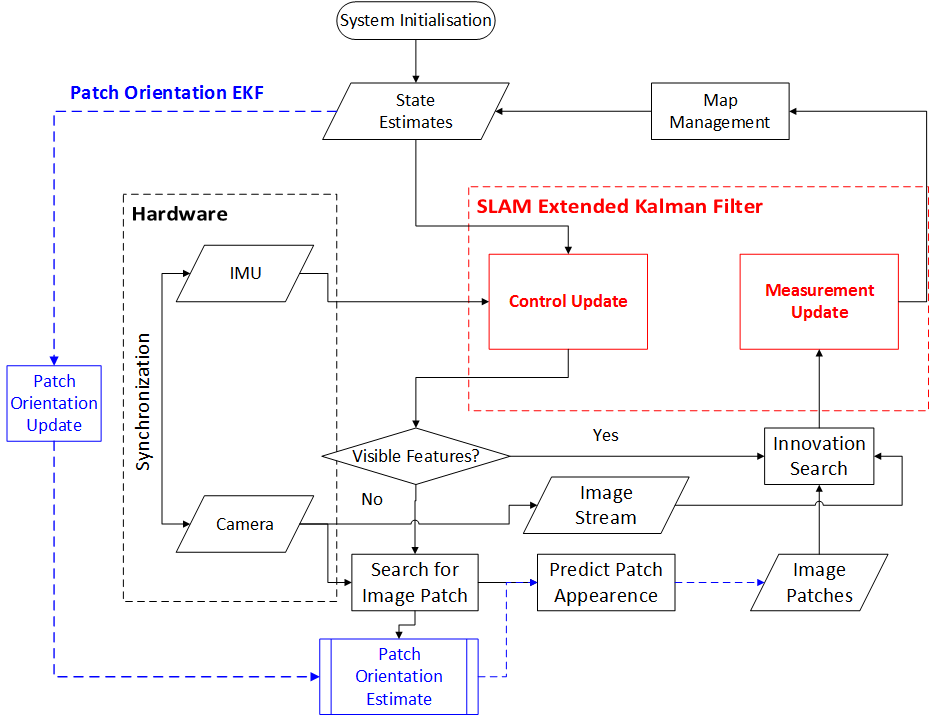
\includegraphics[width=\textwidth, height=0.8\textwidth]{Figures/System.png}
\caption{System functional diagram also depicting the relevant sub-systems.}
\label{fig:system}
%\end{center}
\end{figure}
%%%%%%%%%%%%%%%%%%%%%%%%%%%%%%%%%%%%%%%%%%%%%%%%%%%%%%%%%%%%%%%%%%%%%%%%%%
\newpage
\subsection{State Representation}
As previously mentioned, state variables represent the mathematical ``state" of system. In order to calculate a belief distribution, the system must possess a model to predict future states. This model previously discussed as the state transition probability is commonly referred to as the \textit{motion model}. All relevant states are embedded within the state vector $\textbf{{x}}_t$. The state vector is defined at each time-step and comprises of the robot's \textit{actual} pose and the \textit{actual} landmark positions within the map.\\
Mathematically, the probabilistic map is typically represented as a state \textit{estimate} comprised of a mean state vector $\boldsymbol{\mu}_t$ and a covariance matrix $\boldsymbol{\Sigma}_{t}$, the subscript $t$ denotes a particular time-instance. The mean state vector, is a single column vector containing the estimates of the robot as well as the landmark positions, and the covariance matrix is a square matrix containing the covariances of each state with respect to every other state. These quantities can be mathematically shown according to the book Probabilistic Robotics by Thrun et al.~\cite{probrob}:

\begin{equation}
\boldsymbol{\mu}_t = 
 \begin{pmatrix}
  \textbf{{x}}_{v,t}\\
  \textbf{{y}}_{1,t} \\ 
  \textbf{{y}}_{2,t} \\
  \vdots \\
  \textbf{{y}}_{n,t}
 \end{pmatrix} , \hspace{0.5cm}
\boldsymbol{\Sigma}_{t} =
 \begin{pmatrix}
  {\Sigma}_{x,x} & {\Sigma}_{x,{y_1}} & {\Sigma}_{x,{y_2}} & \cdots & {\Sigma}_{x,{y_N}} \\
  {\Sigma}_{{y_1},x} & {\Sigma}_{{y_1},{y_1}} & {\Sigma}_{{y_1},{y_2}} & \cdots &  {\Sigma}_{{y_1},{y_N}} \\
  {\Sigma}_{{y_2},x} & {\Sigma}_{{y_2},{y_1}} & {\Sigma}_{{y_2},{y_2}} & \cdots &  {\Sigma}_{{y_2},{y_N}} \\
  \vdots  & \vdots  & \vdots & \ddots & \vdots  \\
  {\Sigma}_{{y_n},x} & {\Sigma}_{{y_n},{y_1}} & {\Sigma}_{{y_n},{y_2}}& \cdots & {\Sigma}_{{y_n},{y_N}}
 \end{pmatrix}.
\end{equation}
These quantities then, allow us to approximate the uncertainty regarding the generated feature map as a $N$-dimensional single multi-variate Gaussian distribution, where $N$, as stated above, is the total number of state estimates within the state vector and $n$ is the total number of landmarks within the map.
\begin{wrapfigure}{l}{0.5\textwidth}
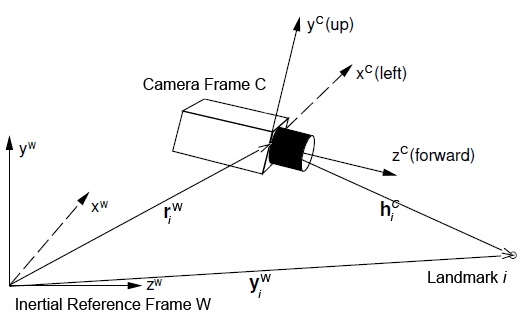
\includegraphics[width=\linewidth,height=5cm]{Figures/frames_mac.png}
\caption{Graphical representation of the appropriate reference frames. Adapted from~\cite{dav2007}}
\label{fig:frame}
\end{wrapfigure}
%%%%%%%%%%%%%%%%%%%%%%%%%%%%%%%%%%%%%%%%%%%%%%%%%%%%%%%%%%%%%%%%%%%%%%%%%%
\subsubsection{Position State Representation}
The camera position state $\textbf{x}_v$ represents all relevant information regarding the camera's position and orientation in a 3D space. The position state vector is comprised of the 3D position vector, $\textbf{{r}}^W$, the unit orientation \textit{quaternion} $\textbf{{q}}^{WC}$ and the linear velocity vector, $\textbf{V}^W$ representing the first derivatives of the position vector. The state camera vector - comprising of 10 individual states - is mathematically described as follows:
\begin{equation}
\textbf{{x}}_v=  
 \begin{pmatrix}
  \textbf{{r}}^W\\
  \textbf{{q}}^{WC} \\ 
  \textbf{{v}}^W\\
 \end{pmatrix} ,
\end{equation}
where $\textbf{r}^W =$ (\textit{x} \textit{y} \textit{z}$)^T$ indicates the 3D cartesian position of the camera, $\textbf{{q}}^{WC}$ the unit orientation \textit{quaternion} indicating the camera orientation (represented in the body frame $C$) relative to the inertial reference frame $W$ while $\textbf{{v}}^W$ indicates the \textit{linear} velocities of the camera relative to the inertial reference frame $W$. The reference frames are depicted in Figure~\ref{fig:frame}.

A quaternion, as previously mentioned, represents the camera's orientation. Quaternions are chosen as opposed to Euler angles to prevent the scenario where one degree of freedom is lost due to two axes driven in a parallel configuration. This scenario is more commonly referred to as a \textit{gimbal lock}. It should be noted that all quaternions represented in this paper are unit quaternions. This implies that the square root of the sum of all the squared elements is always equal to 1:
\begin{equation}
\textit{q}_{0,t}^2 + \textit{q}_{1,t}^2 + \textit{q}_{2,t}^2 + \textit{q}_{3,t}^2 = 1.
\end{equation}
When considering a rotation that changes a robot's orientation, the process of computing the quaternion involves obtaining an angle-axis as well as a magnitude by which this axis is to be rotated. This process is described later in this chapter with reference to the state transition model.

Often, the modelling of dynamic systems require that additional parameters - apart from those describing the position and orientation of the robot - be included in the state vector along with the position state vector. This is illustrated in the description above, with the linear velocity vector, $\textbf{V}^W$, forms the additional information required for system modelling. This is due to the control inputs, which are of such a nature that intermediary state (namely the linear velocity) is required to describe the control inputs effect on the actual position. 
%%%%%%%%%%%%%%%%%%%%%%%%%%%%%%%%%%%%%%%%%%%%%%%%%%%%%%%%%%%%%%%%%%%%%%%%%%

%%%%%%%%%%%%%%%%%%%%%%%%%%%%%%%%%%%%%%%%%%%%%%%%%%%%%%%%%%%%%%%%%%%%%%%%%%   
\subsubsection{Feature Representation}
As previously discussed, the aim is to describe a set of high-quality, well defined landmarks within the map. The map itself is to contain a 3D position of \textit{each} observed landmark  as well as a combined uncertainty. The feature estimates $\textbf{{y}}_n$ - comprising of $N$ landmarks - is mathematically described through three individual cartesian coordinates - $x$, $y$ and $z$ respectively:
\begin{equation}
\textbf{{y}}_n = (x_n\hspace{0.25cm}y_n\hspace{0.25cm}z_n)^T,
\end{equation}
where $n$ corresponds to a specific, single landmark.
%\textcolor{red}{With reference to the theory on image processing, it can be discussed that the depth of a given landmark (in this case the $z$-coordinate) cannot be immediately determined, but rather approximated via triangulation given the landmark is observed over a sequence of (minimally) two known camera positions. The $x$ and $y$ measurements however, can be immediately determined from the image plane.}
\newpage
%%%%%%%%%%%%%%%%%%%%%%%%%%%%%%%%%%%%%%%%%%%%%%%%%%%%%%%%%%%%%%%%%%%%%%%%%%
\subsubsection{Measurement Sensor: Camera} \label{sec:cam}
The measurement sensor of the the robot in this instance is a single CMOS digital camera. The camera is modelled using the \textit{pinhole camera model} depicted in Figure~\ref{fig:pinhole}. The pinhole model provides a reasonable approximation of a 3D point in the world and approximates this position according to a 2D. This model incorporates certain assumptions - namely that most digital cameras use lenses rather than a pinhole that can result in distortion. The model can however be adapted to account for the assumption and better approximate the distortion.

The pinhole camera model can be described as a two-dimensional plane, containing the projections of the 3D point $P_i = (x_i\hspace{0.2cm} y_i\hspace{0.2cm}z_i)^T$. The process of representing a 3D coordinate in terms of a 2D coordinate $Q_i = (u_i\hspace{0.2cm}v_i)^T$ is known as \textit{perspective projection}. The 2D plane is commonly referred to as the \textit{pinhole plane} which contains a infinitesimal hole at its centre - the \textit{pinhole}. The camera possess its own 3D coordinate system with coordinate axes $X_C$, $Y_C$ and $Z_C$ (also referred to as the camera's \textit{optical axis}). The pinhole is situated at the origin of this 3D coordinate system - this is also referred to as the \textit{optical centre}, \textit{O}. The \textit{image plane} is located at a positive distance \textit{f} from the optical centre \textit{O}, parallel to the pinhole plane. This distance $f$ is referred to as the camera's \textit{focal length}.     
\begin{figure}[h]
\begin{center}
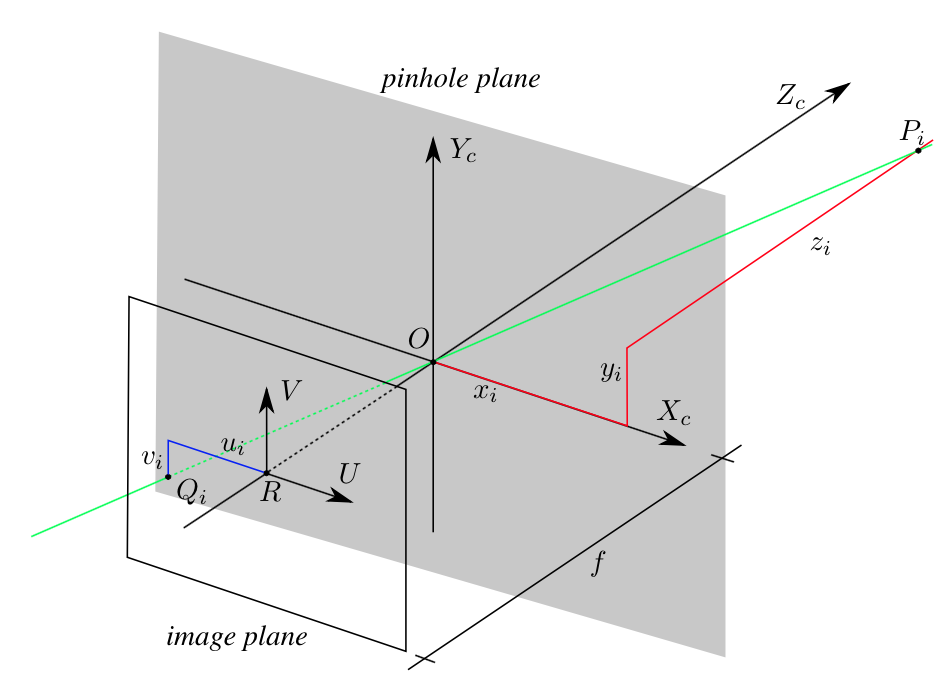
\includegraphics[width=0.9\textwidth, height=0.45\textwidth]{Figures/1.png}
\caption{The pinhole camera model. The red lines show the displacement of a point $P_i$ from the optical centre, the blues line show the displacement of a point $Q_i$ from the image centre and the green line shows the projection from the point $P_i$ point $Q_i$. Adapted from~\cite{master}}
\label{fig:pinhole}
\end{center}
\end{figure}

The undistorted projection of a point $P_i$ in the image plane ($u_i$,$v_i$) can be shown as presented in a thesis by Albrecht~\cite{master}:
\begin{equation} 
\label{eq:fmmd1}
  \begin{pmatrix}
  u_i\\
  v_i\\
  1
  \end{pmatrix} =
  \begin{pmatrix}
  f & 0 & u_0\\
  0& f  & v_0\\
  0& 0 & 1 
  \end{pmatrix}
  \begin{pmatrix}
  \frac{u_i}{f} \\
  \frac{v_i}{f} \\
  1
  \end{pmatrix}
  =  \textbf{C}
  \begin{pmatrix}
  \frac{u_i}{f} \\
  \frac{v_i}{f} \\
  1
  \end{pmatrix},
\end{equation}
where $\textbf{C}$ represents the camera's \textit{intrinsic matrix}, $u_0$ and $v_0$ represents the \textit{principal point} located at the image centre.

As previously mentioned, the pinhole camera model is an approximation of the CMOS machine vision camera that is actually being used. To account for the errors that such an approximation may yield, it is proposed that the \textit{projected} coordinates ($u_i,v_i$) be warped with a \textit{radial distortion} as is done in~\cite{dav2007}, in order to obtain a new \textit{distortion} coordinate ($u_d, v_d$) that will better resemble the one which the camera will provide. This radial distortion is mathematically shown as in a study presented by Swaminathan and Kayer~\cite{distort}:
\begin{equation} \label{eq:raddist}
\begin{split}
u_d - u_0 &= \frac{u-u_0}{\sqrt{1+2K_1r^2}} \\
v_d - v_0 &= \frac{v-v_0}{\sqrt{1+2K_1r^2}}, \\
r &= \sqrt{(u - u_0)^2+(v-v_0)^2},
\end{split}
\end{equation}
where $K_1$ and $r$ represent the radial distortion parameters. 
\newpage
%%%%%%%%%%%%%%%%%%%%%%%%%%%%%%%%%%%%%%%%%%%%%%%%%%%%%%%%%%%%%%%%%%%%%%%%%%
\subsubsection{Control Input Equivalent}\label{sec:imu}
%\textbf{Still reading up on some literature before properly defining this section}
The following concept describes the dynamics to the system as a result of external influences. Upon considering the original MonoSLAM approach, it is evident that there are no \textit{observable} control inputs. The approach presented in this paper though, aims to use measurements obtained through an IMU as an equivalent control input in order to derive a motion model that is potentially more accurate than the implementation of Davison et. al~\cite{dav2007}.

In most instances of robotics, it is essential to describe the dynamics involving a robot's movement. In the context of this paper, the robot/camera is free to move freely as per the user's control requests. Evidently, these requests exert external dynamics upon the system which are uncertain and stochastic at best.

In the approach presented by Davison et al., a constant velocity model is assumed and at each time-step, unknown linear and angular acceleration zero-mean, Gaussian processes are introduced that cause linear and angular velocity impulses. The model contains very little, if any information on the movement of the camera. It can be assumed that utilising additional information regarding the camera's movement will provide greater accuracy upon state estimation.

The inertial sensors, in the form of an IMU, is ideally mounted onto the camera. This allows the camera to be modelled as a rigid body upon which a kinematic estimation can be applied. The IMU directly measures the total accelerations $\textbf{f}_t$ as well as the angular rates $\boldsymbol{\omega}_t$ with respect to the cameras rigid body frame $C$.

The control vector equivalent however, requires that the linear portion of the acceleration be obtained from the IMU measurement. It is known that the total acceleration measured by the IMU's accelerometer is adapted from a study presented by Servent et. al~\cite{IMU}:

\begin{equation}
\textbf{f}_t = \textbf{\text{R}}^{CW}(\textbf{a}_t - \textbf{g}),
\end{equation}
with $\textbf{a}_t$ is the linear acceleration vector, $\textbf{g}$ is the gravity vector and $\textbf{\text R}^{CW}$ is the rotation matrix that transforms the camera's body coordinate frame $C$, into the inertial reference frame $W$.\\The rotation matrix is defined according to~\cite{models}:
\begin{equation}
\textbf{R}^{CW} = 
\begin{pmatrix}
q_{0,t}^2+q_{x,t}^2-q_{y,t}^2-q_{z,t}^2 & 2(q_{x,t}q_{y,t}-q_{0,t}q_{z,t}) & 2(q_{x,t}q_{z,t}-q_{0,t}q_{y,t}) \\ 
2(q_{x,t}q_{y,t} +q_{0,t}q_{z,t}) & q_{0,t}^2-q_{x,t}^2-q_{y,t}^2-q_{z,t}^2 & 2(q_{y,t}q_{y,z}-q_{0,t}q_{x,t}) \\ 
2(q_{x,t}q_{z,t}-q_{0,t}q_{y,t}) & 2(q_{y,t}q_{z,t}+q_{0,t}q_{x,t}) & q_{0,t}^2-q_{x,t}^2-q_{y,t}^2+q_{z,t}^2 \\ 
\end{pmatrix}.
\end{equation}

The linear acceleration is a processed measurement from the directly obtained accelerometer measurement. The accelerometer measurements firstly subtract the gravity vector $\textbf{g}$ before being rotated according to the correct orientation frame (from $C$ to $W$).

Once obtained, these measurements  form the \textit{equivalent control vector} $\textbf{u}_t$ that describes, at each time-step, the dynamics of the system as a result of external forces. The control vector equivalent is adapted as follows:

\begin{equation}
\textbf{u}_t =
\begin{pmatrix} 
 \textbf{a}_t \\
 {\boldsymbol \omega}_t
\end{pmatrix}
= \begin{pmatrix}\hspace{0.1cm}\ddot{x}_{t}\hspace{0.25cm}\ddot{y}_{t}\hspace{0.25cm}\ddot{z}_{t}\hspace{0.25cm}{\omega}_{x,t}\hspace{0.25cm}{\omega}_{y,t}\hspace{0.25cm}{\omega}_{z,t}\hspace{0.1cm}
\end{pmatrix}^T.
\end{equation}

Because the IMU measures the actual movements through sensors, namely an accelerometer and a gyroscope, it is important to note the effects of disturbances and process noise can be directly obtained through these measurements. Moreover, the uncertainty regarding the transition model, namely the process noise, is all incorporated within the noise measurements of the IMU. This noise can be modelled as a zero mean, Gaussian process $\textbf{w}_t$ with a corresponding covariance matrix $\textbf{R}_w$. The system noise can be then be mathematically described as follows:
 
\begin{equation} \label{eq:pertn}
\textbf{w}_t =
\begin{pmatrix} 
 \textbf{n}_{\textbf{a},t} \\
 \textbf{n}_{{\omega},t}
\end{pmatrix}
= \begin{pmatrix}\hspace{0.1cm}n_{\ddot{x}_{t}}\hspace{0.25cm}n_{\ddot{y}_{t}}\hspace{0.25cm}n_{\ddot{z}_{t}}\hspace{0.25cm}n_{{\omega}_{x,t}}\hspace{0.25cm}n_{{\omega}_{y,t}}\hspace{0.25cm}n_{{\omega}_{z,t}}\hspace{0.1cm}
\end{pmatrix}^T,
\end{equation}
with the aforementioned noise model is assumed to be a Gaussian random variable for each of the above elements.  

Furthermore, the resultant IMU data to be used is to contain the measurements of the linear accelerations and angular rotations as well as the appropriate additive noise.
%%%%%%%%%%%%%%%%%%%%%%%%%%%%%%%%%%%%%%%%%%%%%%%%%%%%%%%%%%%%%%%%%%%%%%%%%%
\newpage
\subsection{Control Update}
This section presents the necessary steps to incorporate the control update of the EKF.

With reference to the probabilistic form of the solution to the SLAM problem, the prediction step requires a description in terms of a belief distribution. The description of the aforementioned state transition model can then, in terms of the probability distribution on the state transitions, take the following form:
\begin{equation}
\begin{split}
p(\textbf{{x}}_t\hspace{0.15cm}|\hspace{0.15cm}\textbf{{x}}_{t-1}, \textbf{u}_t)&=\cfrac{1}{\sqrt{|2\pi\textbf{R}_w|}}\hspace{0.1cm}\text{exp}\hspace{0.1cm}\bigg\{ \frac{1}{2}\big[\textbf{{x}}_t-g(\boldsymbol{\mu}_t, \hspace{0.1cm}\boldsymbol{\mu}_{t-1}) - \textbf{G}_t^{x_t}(\textbf{x}_{t-1} - \boldsymbol{\mu}_{t-1})\big]^T\\
\textbf{R}^{-1}_w&\big[\textbf{{x}}_t-g(\boldsymbol{\mu}_t, \hspace{0.1cm}\boldsymbol{\mu}_{t-1}) - \textbf{G}_t^{x_t}(\textbf{x}_{t-1} - \boldsymbol{\mu}_{t-1})\big]\bigg \},
\end{split},
\end{equation} 
where $\textbf{G}_t^{x_t}$ represents the Jacobian of the state transition motion and $\textbf{R}_w$ is the process noise. \\\\
The state transition model is assumed to take the form of a Markov process, yielding that the current state $\textbf{{x}}_{t}$ is only dependent upon the state immediately preceding it - $\textbf{{x}}_{t-1}$ - as well as the input control $\textbf{{u}}_t$. Additionally, it is important to note that the uncertainty regarding the state transition model is independent of the uncertainty regarding both the observation model as well as that of the probabilistic map itself.
%%%%%%%%%%%%%%%%%%%%%%%%%%%%%%%%%%%%%%%%%%%%%%%%%%%%%%%%%%%%%%%%%%%%%%%%%%
%%%%%%%%%%%%%%%%%%%%%%%%%%%%%%%%%%%%%%%%%%%%%%%%%%%%%%%%%%%%%%%%%%%%%%%%%%
\subsubsection{State Transition Model} 
As previously discussed, the EKF requires a state transition (motion) model in order to obtain the mean estimate $ \boldsymbol{\bar \mu}_t$, of  current state of the system. In short, the motion model describes the transition from the previous state to the following state with regard to the robot�s kinematic motion as well as the control inputs. In order to derive the state transition model for the system at hand, it is vital that the certain characteristics of the system be understood. Firstly, the robot system - from here on in to be referred to as the \textbf{camera} - is comprised of a monocular camera and an attached IMU package. Secondly, the camera is to be considered as a six degree of freedom (DOF) rigid body. Briefly the six DOF describe the camera's three \textit{translational} and three \textit{rotational} degrees of freedom. 

We therefore set out to define a kinematic estimation based motion model - using Newton's laws of motion - to describe the camera's movement through the environment as a result of initially unknown, external inputs to the system. Lastly, it should be stressed that embedded within the motion model should be the impacts of uncertainty through both internal and external factors.

It must be stressed that a derivation for the suitable motion model will obtained before a first order Taylor approximation is obtained as required by the EKF. Recalling, the states and control inputs:

\begin{equation}
\begin{split}
\textbf{x}_t &=
\begin{pmatrix}
\hspace{0.1cm}\textbf{r}_t^{W}\hspace{0.1cm}\textbf{q}_t^{WC}\hspace{0.1cm}\textbf{v}_t^{W}
\end{pmatrix}^T\\ 
%&=\begin{pmatrix}
%\textit{x}_{t}\hspace{0.25cm}\textit{y}_{t}\hspace{0.25cm}\textit{z}_{t}\hspace{0.25cm}\textit{q}_{0,t}\hspace{0.25cm}\textit{q}_{1,t}\hspace{0.25cm}\textit{q}_{2,t}\hspace{0.25cm}\textit{q}_{3,t}\hspace{0.25cm}\textit{\.{x}}_{t}\hspace{0.25cm}\textit{\.{y}}_{t}\hspace{0.25cm}\textit{\.{z}}_{t} 
%\end{pmatrix}^T\\
\textbf{u}_t
&=\begin{pmatrix}
\hspace{0.1cm}\textbf{a}_t^C\hspace{0.1cm}\boldsymbol{\omega}_t^C
\end{pmatrix}^T\\
%&=\begin{pmatrix}
%\hspace{0.1cm}\ddot{x}_{t}\hspace{0.25cm}\ddot{y}_{t}\hspace{0.25cm}\ddot{z}_{t}\hspace{0.25cm}{\omega}_{x,t}\hspace{0.25cm}{\omega}_{y,t}\hspace{0.25cm}{\omega}_{z,t}\hspace{0.1cm}
%\end{pmatrix}^T\\
\end{split}.
\end{equation}
\\\\
Considering that the EKF is a recursive, numerical evaluation, it is necessary to convert the \textit{continuous} linear differential equations that describe the state transition model into a discrete counterpart. Various methods of discretisation exist, though this specific implementation makes use of the forward difference (Euler�s) method as the sampling period is assumed to be small enough. This method \textit{approximates} the derivative for a state for a sampling period $\Delta T$ as follows:  
\begin{equation}
\begin{split}
\textbf{\.{x}}_{t-1} &= \lim_{\Delta T\to 0}{\frac{\textbf{x}_{t}-\textbf{x}_{t-1}}{\Delta T}} 		 \\										 \textbf{x}_{t} &\approx \textbf{\.{x}}_{t-1}\Delta T + \textbf{x}_{t-1}
\end{split}.
\end{equation}  
Newton's second law of motion, describing the relationship between a body's mass and it's acceleration, is used to derive the linear motion mode after which the aforementioned method of discretisation is applied to obtain the discrete motion model. A full derivation of the linear state transition model is shown in Appendix~\ref{App:Concepts}.

The non-linear state transition function of the kinematic estimator $g(\textbf{u}_{t},\textbf{x}_{t-1})$ is defined at the current time $t$, is dependent on both the current control input equivalents $\textbf{u}_t$ as well as the actual states $\textbf{x}_{t-1}$. The non-linear behaviour is a result of the change in orientation of the camera:
\begin{equation} \label{eq:trmod}
\begin{split}
\textbf{g}(\textbf{u}_{t},\textbf{x}_{t-1}) =
	\begin{pmatrix}
		\textbf{r}_t^{W}\\
		\textbf{q}_t^{WC}\\
		\textbf{v}_t^{W} \\
	\end{pmatrix} &= 
	\begin{pmatrix}
		\textbf{r}_{t-1}^{W}+\textbf{v}_t^W\Delta T\\
		\textbf{q}_{t-1}^{WC} \otimes \text{quat}\big(\boldsymbol{\omega}_t^C\Delta T\big) \\
		\textbf{v}_t^{W} + \textbf{a}_{t}^C \Delta T \\
	\end{pmatrix} \\
&= \begin{pmatrix}
	 \textbf{r}_{t-1}^{W}+\dot{\textbf{r}}^W\Delta T\\
	 \textbf{q}_{t-1}^{WC} \otimes \text{quat}\big(\boldsymbol{\omega}_t^C\Delta T\big) \\
	 \dot{\textbf{r}}_t^{W} + \textbf{R}_t^{CW}\big(\ddot{\textbf{r}}_{t}^C \Delta T\big) \\
\end{pmatrix} \\
\end{split},
\end{equation}
where $\Delta T$ is defined as the sample period between the previous time $t-1$ and $t$ and $\text{quat}\big(\boldsymbol{\omega}_t^C\Delta T\big)$ denotes the process of obtaining a quaternion of the rotation $\boldsymbol{\dot \omega}_t^C\Delta T$. Information regarding the change in linear acceleration is directly obtained from the control input equivalent data gathered by the IMU and can be numerically integrated it obtain linear velocity and ultimately, translational position.\\\\
\textit{All of the equations in the remainder of this subsection are adapted from the MonoSLAM documentation on models provided by Davison}~\cite{models}\\\\
In order to compute the aforementioned quaternion, the rate at which the camera's rotational degrees of freedom are changing is required. The control input equivalent measurements from the gyroscope however, measure exactly this quantity - the angular rate. The angular rate is subsequently numerically integrated in order to obtain the angular position $\boldsymbol{\theta}_t$, before the quaternion is taken thereof. As previously mentioned, an angle-axis as well as a magnitude by which this axis is to be rotated is required to compute a quaternion. The angle-axis $\boldsymbol{\gamma}$ is defined as follows:
\begin{equation} \label{eq:axis}
\begin{split}
\boldsymbol{\gamma} &= \begin{pmatrix}
\boldsymbol{\theta}, {\norm{\boldsymbol{\theta}}} 
\end{pmatrix} =
\begin{pmatrix}
\begin{pmatrix}
\theta_x \\
\theta_y \\
\theta_z 
\end{pmatrix}, \norm{\boldsymbol{\omega}_t^C \Delta T} 
\end{pmatrix} = 
\begin{pmatrix}
\begin{pmatrix}
\frac{\omega_{t,X}^C \Delta T}{\norm{\boldsymbol{\omega}_t^C \Delta T}} \\
\frac{\omega_{t,Y}^C \Delta T}{\norm{\boldsymbol{\omega}_t^C \Delta T}} \\
\frac{\omega_{t,Z}^C \Delta T}{\norm{\boldsymbol{\omega}_t^C \Delta T}}  
\end{pmatrix}, \norm{\boldsymbol{\omega}_t^C \Delta T} 
\end{pmatrix}
\end{split},
\end{equation}

where $\omega_{t,\beta}$, $\beta \in \{X, Y, Z\}$ denotes the angular velocity about each respective coordinate axis. The result in Equation~\ref{eq:axis} is then represented as a unit quaternion denoting the same rotation:

\begin{equation} \label{eq:quat} 
\textbf{q} = \bigg(\cos \frac{\alpha}{2} \hspace{0.4cm} \frac{\theta_x}{\norm{\boldsymbol{\theta}}}\sin\frac{\alpha}{2} \hspace{0.4cm} \frac{\theta_y}{\norm{\boldsymbol{\theta}}}\sin\frac{\alpha}{2} \hspace{0.4cm} \frac{\theta_z}{\norm{\boldsymbol{\theta}}}\sin\frac{\alpha}{2} \bigg)^T.
\end{equation}

A quaternion multiplication between the orientation quaternion obtained at the previous time step and the angle-axis rotation quaternion in Equation~\ref{eq:quat} results in the camera's final orientation state at the the current time $t$.
%%%%%%%%%%%%%%%%%%%%%%%%%%%%%%%%%%%%%%%%%%%%%%%%%%%%%%%%%%%%%%%%%%%%%%%%%%
\subsubsection{Mean Estimate}\label{sec:kinest}
The control update uses the previously defined state transition function to obtain a state estimate $\boldsymbol{\bar \mu}_t$ at the current time instance. This procedure is shown in Step 1 of Table~\ref{tab:EKF}. Recalling, the state transition function is dependent on both the current equivalent control inputs as well as the actual states to obtain a suitable state estimate:

\begin{equation} \label{eq:trmod1}
\begin{split}
\textbf{g}(\textbf{u}_{t},\textbf{x}_{t-1}) 
&= \begin{pmatrix}
	 \textbf{r}_{t-1}^{W}+\dot{\textbf{r}}^W\Delta T\\
	 \textbf{q}_{t-1}^{WC} \otimes \text{quat}\big(\boldsymbol{\omega}_t^C\Delta T\big) \\
	 \dot{\textbf{r}}_t^{W} + \textbf{R}_t^{CW}\big(\ddot{\textbf{r}}_{t}^C \Delta T\big) \\
\end{pmatrix} \\
\end{split}.
\end{equation}

It is worthwhile to note that the equivalent control inputs (which are the measurements from the IMU) incorporate the additive noise. This concept is shown in Equation~\ref{eq:pertn}.
%%%%%%%%%%%%%%%%%%%%%%%%%%%%%%%%%%%%%%%%%%%%%%%%%%%%%%%%%%%%%%%%%%%%%%%%%%
\subsubsection{Covariance Update}
Before the control update can be concluded, the covariance matrix $\boldsymbol{\bar \Sigma_t}$, corresponding to the previously determined mean vector $\boldsymbol{\bar \mu_t}$ is required to be updated as a result of the linearisation process undertaken by the EKF. This procedure is denoted in Step 2 of Table~\ref{tab:EKF}. It can be noticed that the previously described Jacobian matrix of $\textbf{g}(\textbf{u}_{t},\textbf{x}_{t-1})$ is thus required to realise this procedure. The Jacobian matrix of $\textbf{g}(\textbf{u}_{t},\textbf{x}_{t-1})$, $\textbf{G}_t^{x_t}$, can be mathematically defined as follows:

\begin{equation} \label{eq:jacG}
\textbf{G}_t^{x_t} = \frac{\partial \textbf{g}(\textbf{u}_{t},\textbf{x}_{t-1})}{\partial \textbf{x}_{t-1}} = \boldsymbol{\mu}_{t-1}
=\begin{pmatrix}
\frac{\partial \textbf{r}^W_t}{\partial \textbf{r}^W_{t-1}} & \boldsymbol{0} & \frac{\partial \textbf{v}^W_{t}}{\partial \textbf{r}^W_{t-1}}\\
\boldsymbol{0} & \frac{\partial \textbf{q}^{WC}_{t}}{\partial \textbf{q}^{WC}_{t-1}} & \boldsymbol{0}  \\
\boldsymbol{0} & \boldsymbol{0} & \frac{\partial \textbf{v}^W_{t}}{\partial \textbf{v}^W_{t-1}}  \\
\end{pmatrix}, 
\end{equation}   
with the non-zero elements of the Jacobian further trivially defined as follows (and according to the model defined in Equation~\ref{eq:trmod}),

\begin{equation}
\frac{\partial \textbf{r}^W_t}{\partial \textbf{r}^W_{t-1}} = \frac{\partial \textbf{v}^W_{t}}{\partial \textbf{v}^W_{t-1}} =
\begin{pmatrix} \label{eq:iden}
1 & 0 & 0\\
0 & 1 & 0\\
0 & 0 & 1\\
\end{pmatrix} = \textbf{I},
\end{equation}
and

\begin{equation} \label{eq:tiden}
\frac{\partial \textbf{r}^W_{t}}{\partial \textbf{v}^W_{t-1}} = 
\Delta T\begin{pmatrix}
1 & 0 & 0\\
0 & 1 & 0\\
0 & 0 & 1\\
\end{pmatrix} = \Delta T\hspace{0.2cm}\textbf{I},
\end{equation}
The specially defined Jacobian with a partial derivative that is taken with respect to a quaternion however, requires a more intricate solution. The process of defining a new quaternion from the measured angular rate $\boldsymbol{\omega}_t^C$ - as denoted in Equation~\ref{eq:trmod} can be more formally defined as follows:

\begin{equation}
\textbf{q}_t^C = \text{quat}(\boldsymbol{\omega}^C_t \Delta T).
\end{equation}
Hereafter, the final non zero element of the Jacobian can be defined in terms of the aforementioned new quaternion: 

\begin{equation}
\frac{\partial \textbf{q}^{WC}_{t}}{\partial \textbf{q}^{WC}_{t-1}} = 
\begin{pmatrix}
 q^C_{1,t}&-q^C_{2,t} & -q^C_{3,t} & -q^C_{4,t}\\
 q^C_{2,t}&  q^C_{1,t} & -q^C_{4,t} &  q^C_{3,t}\\
 q^C_{3,t}&  q^C_{4,t} &  q^C_{1,t} & -q^C_{2,t}\\
 q^C_{4,t}& -q^C_{3,t} &  q^C_{2,t} &  q^C_{1,t} \\
\end{pmatrix}.
\end{equation}
In order to complete the covariance update, the process noise covariance is still required to be updated. Upon revising, the process noise is captured by the control inputs and modelled as a zero-mean Gaussian process. The noise covariance $\textbf{R}_w$ then, can be formally defined as follows:
\begin{equation}\label{eq:proR}
\textbf{R}_w = 
\begin{pmatrix}
n_{\ddot{x},t}& 0 & 0 & 0 & 0 & 0 \\
0& n_{\ddot{y},t} & 0 & 0 & 0 & 0 \\
0& 0 & n_{\ddot{z},t} & 0 & 0 & 0 \\
0& 0 & 0 & n_{\omega_{x},t} & 0 & 0 \\
0& 0 & 0 & 0 & n_{\omega{y},t} & 0 \\
0& 0 & 0 & 0 & 0 & n_{\omega{z},t} \\
\end{pmatrix} ^2,
\end{equation}
with the perturbation levels $n_{w,t}$ as defined in equation~\ref{eq:pertn}.
%%%%%%%%%%%%%%%%%%%%%%%%%%%%%%%%%%%%%%%%%%%%%%%%%%%%%%%%%%%%%%%%%%%%%%%%%%
\newpage
\subsection{Measurement Update}
With reference again to the probabilistic form of the solution to the SLAM problem, the measurement step too, requires a description in terms of a belief distribution. The observation model however, models the uncertainty regarding a measurement taken at any given time instance $\textbf{{z}}_t$, given that the locations of both the robot as well as the location of the landmarks are known. This uncertainty can be described in the following form:  
\begin{equation}
\begin{split}
p(&\textbf{z}_t\hspace{0.1cm}|\hspace{0.15cm}\textbf{x}_{t}) \\
&=\cfrac{1}{\sqrt{|2\pi\textbf{R}_v|}}\hspace{0.1cm}\text{exp}\hspace{0.1cm}\bigg\{ \frac{1}{2}\big[\textbf{{z}}_t-\textbf{h}( \boldsymbol{\bar \mu}_t)-\textbf{H}_t^{x_t}(\textbf{x}_t -  \boldsymbol{\bar \mu}_t)\big]^T \textbf{R}_v^{-1}\big[\textbf{{z}}_t-\textbf{h}( \boldsymbol{\bar \mu}_t)-\textbf{H}_t^{x_t}(\textbf{x}_t -  \boldsymbol{\bar \mu}_t)\big] \bigg\}
\end{split},
\end{equation} 
where $\textbf{H}_t$ represents the Jacobian of the observation model and $\textbf{R}_v$ is the sensor noise. \\\\
It can be (reasonably) assumed that the uncertainty regarding the measurements are conditionally independent given the uncertainty regarding the robot and landmark locations if indeed they are completely defined. Also, the correction step seeks to obtain the difference between the actual measurements $\textbf{{z}}_k$ and the predicted measurements. These predicted measurements are to be obtained through an observation model that we from hereon in refer to as the measurement function, denoted as $\textbf{h}(\boldsymbol{\bar \mu})$.  
%%%%%%%%%%%%%%%%%%%%%%%%%%%%%%%%%%%%%%%%%%%%%%%%%%%%%%%%%%%%%%%%%%%%%%%%%%
%\subsubsection{}
%%%%%%%%%%%%%%%%%%%%%%%%%%%%%%%%%%%%%%%%%%%%%%%%%%%%%%%%%%%%%%%%%%%%%%%%%%
\subsubsection{Measurement Model}
The correction step of the EKF aims to ultimately correct the previously estimated robot pose and landmark position through exterior sensor measurements. With regard to the implementation proposed in this paper, these measurements are obtained through the use of a camera. The measurement process generally involves a measurement estimate that incorporates uncertainty.\\

With reference to figure~\ref{fig:frame}, a feature's cartesian position can be described through a cartesian vector $\textbf{h}^W_i(\boldsymbol{\bar \mu})$, where the feature's cartesian \textbf{point} is shown in relation to the camera's centre: 

\begin{equation}
\textbf{h}^W_{i}(\boldsymbol{\bar \mu}) = \textbf{R}^{CW}\big(\textbf{y}^W_{i}-\textbf{r}^W\big) = 
  \begin{pmatrix}
  \begin{pmatrix}
  x_{i}\\
  y_{i} \\ 
  z_{i} \\
  \end{pmatrix} - \textbf{r}^{W} 
  \end{pmatrix}  
\end{equation}
the subscript $i$ corresponds a directional vector $\textbf{h}^C$ from it's cartesian position $\textbf{r}^W$ to the cartesian position of a given landmark $\textbf{y}^W$.\\\\
A camera however, cannot directly measure a cartesian vector. Instead, a camera measurement (based on the model presented) obtains a vector $\textbf{h}_i$ that is a function of $\textbf{h}^W_{i}$. This vector describes a given feature's horizontal and vertical image positions $(u,v)$. For an undistorted image, the vector $\textbf{h}_i$, more commonly referred to as the measurement function is defined according to Equation~\ref{eq:fmmd1}:

 \begin{equation} \label{eq:fmmd}
\textbf{h}_i = 
  \begin{pmatrix}
  u_i \\
  v_i \\ 
  \end{pmatrix} =
    \begin{pmatrix}
  u_0 - fk_u\cfrac{h^R_{i,x}}{h^R_{i,z}}\\
  v_0 - fk_v\cfrac{h^R_{i,y}}{h^R_{i,z}} \\ 
  \end{pmatrix} 
\end{equation}

where $u_0$ and $v_0$ represent the principal point and $fk_u$ and $fk_v$ are the camera calibration parameters described in Chapter~\ref{sec:cam}.

It is evident from the model presented in equation~\ref{eq:fmmd} cannot be directly inverted to obtain a feature's position. The projection of a feature onto the camera's image plane removes any information required to directly obtain the depth of the feature.  

%%%%%%%%%%%%%%%%%%%%%%%%%%%%%%%%%%%%%%%%%%%%%%%%%%%%%%%%%%%%%%%%%%%%%%%%%%
%\subsubsection{Feature Tracking}
\subsubsection{Feature Matching}
The following section discusses the measurement of a feature \textit{fully} initialised within the SLAM map. The measurement process seeks to initially estimate the cartesian position of a given feature $\textbf{y}_i$ within the SLAM map. Thereafter, the feature can be compared via a matching sequence. Generally, feature matching is conducted using a normalised cross-correlation search, where a 2D template of the 3D feature is scanned is across the entire image (at each pixel location) until a peak is obtained. MonoSLAM however, seeks to utilise an \textit{active} approach for matching, minimising the the search field and improving efficiency.\\
The EKF inherently contains information that may be utilised in order to prohibit a full cross-correlation search. The measurement function $\textbf{h}({\bar\mu})$ for instance, provides an estimate for a given features location, namely $\textbf{u}_d = ({u}_d,v_d)$. Knowledge of this location therefore allows an active search region to be described within the vicinity of this location. The location estimate of the feature is not the only information regarding the feature that is available as a result of the EKF. Additionally, the uncertainty regarding a given feature's location is stored within the state vector covariance matrix $\textbf{P}_{nN}$. This information can be used to determine the size of the active search region surrounding the location estimate; where the size of the search region is directly proportional to the uncertainty of it's location. If the feature cannot be matched within the aforementioned search region, it cannot contribute to the correction of the robot's pose estimate and is therefore deleted form the SLAM map. The aforementioned process of defining the active search region can be mathematically defined through the \textit{innovation covariance matrix} $\textbf{S}_i$:
\begin{equation}\label{eq:inov}
%\begin{split}
\textbf{S}_i = \frac{\partial\textbf{u}_{d,i}}{\partial\textbf{x}_{v}}\Sigma_{\textbf{x}_v,\textbf{x}_v}\frac{\partial\textbf{u}_{d,i}}{\partial\textbf{x}_{v}}^T + \frac{\partial\textbf{u}_{d,i}}{\partial\textbf{x}_{v}}\Sigma_{\textbf{x}_vy_i}\frac{\partial\textbf{u}_{d,i}}{\partial\textbf{y}_{i}}^T + \frac{\partial\textbf{u}_{d,i}}{\partial\textbf{y}_{i}}\Sigma_{y_i\textbf{x}_v}\frac{\partial\textbf{u}_{d,i}}{\partial\textbf{x}_{v}}^T + \frac{\partial\textbf{u}_{d,i}}{\partial\textbf{y}_{i}}\Sigma_{y_iy_i}\frac{\partial\textbf{u}_{d,i}}{\partial\textbf{y}_{i}}^T + \textbf{R}_v
%\end{split}
\end{equation}
The symmetric $2\times2$ matrix $\textbf{S}_i$ represents a 2D Gaussian PDF around the estimated image coordinate. The innovation covariance matrix can then be used to determine an active region the a given feature should lie within. Typically, the active search region is defined to confine within 3 standard deviations (3$\sigma$) of the mean.\\
Furthermore, the innovation matrix provides a measure of the amount of content expected within an eventual actual measurement $\textbf{z}_i$. In the event that many potential measurements are available, features containing a higher $\textbf{S}_i$ present the EKF with more information regarding the camera's position. Candidates for feature estimates are thus chosen according to those that present the most information regarding the position estimate. Feature searches per sampling instance are generally limited (usually about 12 features) due to computational constrains.\\         
Finally, as described in~\cite{dav2007}, an active search will always reduce the area of the template matching search region at the potential \textit{additional} cost of calculating the reduced search region.
%%%%%%%%%%%%%%%%%%%%%%%%%%%%%%%%%%%%%%%%%%%%%%%%%%%%%%%%%%%%%%%%%%%%%%%%%%
\subsubsection{Feature Initialisation}
The inherent disadvantage of a monocular camera, as previously mentioned, is the inability to immediately provide an estimate for the depth of a feature. As a result, a given feature is required to be observed at various viewpoints before its depth can be approximated through a multiple view triangulation. Instead, Davison et al. presents an alternative approach whereby a feature is initialised to lie along an infinite 3D line. This line, originating from the position at which the camera is estimated, extends indefinitely in the direction of the feature. The depth of the feature lies somewhere along the aforementioned line. This depth can be modelled as a uniformly distributed set of discrete depth hypothesis. Briefly, the feature's depth can be interpreted as a 1D probability density, represented only by particle distribution instead. The feature is can then \textit{partially} initialised in the SLAM map as follows:
\begin{equation}
\textbf{y}_{pi} =
\begin{pmatrix}
\textbf{r}_{i}^W \\
 \textbf{\^{h}}_{i}^W \\
\end{pmatrix}
\end{equation}
where $\textbf{r}_{i}^W$ represents the origin of the line and $\textbf{\^{h}}_{i}^W$ is a unit vector representing its direction. The uncertainty describing the aforementioned entities are Gaussian in nature.\\\\
After a feature has been partially initialised, it can be assumed that the feature is re-observed and that each additional observation improves the depth estimate. The particle filter based depth estimation process itself is to a large extent complex, and is explained in more detain in ~\cite{dav2007}. Intuitively, the depth estimation process can be explained as follows: each particle in the particle set is projected into the image and subsequently matched across each observation. The resulting observations transform the initially uniformly distributed depth probability into one that better resembles a Gaussian density. Once the depth covariance is below a certain threshold, the depth is approximated with a Guassian probability density. Thereafter a feature becomes \textit{fully} initialised, assigned with a standard 3D Gaussian representation.
%%%%%%%%%%%%%%%%%%%%%%%%%%%%%%%%%%%%%%%%%%%%%%%%%%%%%%%%%%%%%%%%%%%%%%%%%%
\subsubsection{Map Management}
Map management forms an integral role in the realisation of the MonoSLAM algorithm. A real-time algorithm, as proposed in this paper, relies on efficient and accurate decisions regarding features within the SLAM map. As a result, a strict protocol is followed in~\cite{dav2007} in order to realise a successful real-time algorithm.
%%%%%%%%%%%%%%%%%%%%%%%%%%%%%%%%%%%%%%%%%%%%%%%%%%%%%%%%%%%%%%%%%%%%%%%%%%
%\subsubsection{System Update}
%%%%%%%%%%%%%%%%%%%%%%%%%%%%%%%%%%%%%%%%%%%%%%%%%%%%%%%%%%%%%%%%%%%%%%%%%%
\newpage
%%%%%%%%%%%%%%%%%%%%%%%%%%%%%%%%%%%%%%%%%%%%%%%%%%%%%%%%%%%%%%%%%%%%%%%%%%
\section{Implementation}
\subsection{Introduction}
This chapter sets out to test all the relevant sub-systems incorporated within this project. Initially, the necessary configuration and procedures are given in order to set up the system. Thereafter, the hardware components are individually tested and analysed to ensure that the expected performance is provided and whether redesign is necessary. Lastly, the core of this project, the kinematic estimator, is simulated and analysed as a possible alternative to the current velocity and angular velocity model. 
%%%%%%%%%%%%%%%%%%%%%%%%%%%%%%%%%%%%%%%%%%%%%%%%%%%%%%%%%%%%%%%%%%%%%%%%%%
\subsection{System Setup}
%%%%%%%%%%%%%%%%%%%%%%%%%%%%%%%%%%%%%%%%%%%%%%%%%%%%%%%%%%%%%%%%%%%%%%%%%%
An overview of the system is depicted in Figure~\ref{fig:sys}. It is evident that the system contains three hardware sub-systems:
\begin{itemize}
\item IMU.
\item CMOS Camera.
\item Arduino micro-controller.
\end{itemize}
Each of of the sub-systems requires a unique setup configuration in order to represent a \textit{functional} unit of the whole system.   
%%%%%%%%%%%%%%%%%%%%%%%%%%%%%%%%%%%%%%%%%%%%%%%%%%%%%%%%%%%%%%%%%%%%%%%%%%
\subsubsection{Inertial Measurement Unit}
It can be recalled that inertial measurements are required in order to realise the kinematic estimator described in section~\ref{sec:kinest}. A 6DOF IMU board is thus required to realise these measurements. A 6DOF IMU requires measurements from an accelerometer and a gyroscope. Important properties to be considered upon choosing suitable IMU are as follows:
\begin{itemize}
\item Communication with a master device (in this case a micro-controller).
\item Suitable range that the sensors are capable of measuring.
\item Noise on sensors.
\item Communication speed.
\item Low pass filter to prevent aliasing.
\item Sample code.
\end{itemize}

The 6DOF IMU board to be used in this implementation is the SparkFun 6 DOF IMU as depicted in Figure~\ref{fig:imu}. This board is comprised of a ITG3200 MEMS 3-axis gyroscope~\cite{gyro} and a ADXL345 3-axis linear accelerometer~\cite{acc}. This component is chosen as it contains both the necessary sensors on the same chip while supporting I2C communication, low pass filtering, suitable range, sample code and a maximum sample rate of 1 kHz. Alternative products generally contain an additional 3 DOF and greater ranges that are overlooked considering that these products are generally twice the price of the chosen component. 
\newpage
The IMU is configured with the following properties:

\begin{enumerate}
\item 3.3 Volt input.
\item I2C interface (this device serves as the \textit{slave}).
\item $\pm 2000^{\circ}$ per second range for the gyroscope.
\item $\pm 4 g$ range and 10-bit resolution for the accelerometer.
\item 100 Hz sample rate with 50 Hz Low Pass/Anti Aliasing Filter.
\end{enumerate}
The accelerometer and gyroscope are configured in such a way that the sampling frequency is at least twice the bandwidth of the data (Nyquist frequency) to prevent Aliasing.

\begin{figure}[h]
%\begin{center}
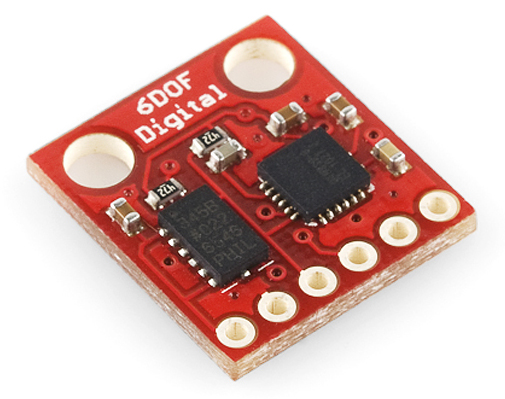
\includegraphics[width=0.49\textwidth, height=0.25\textwidth]{Figures/imu1.jpg}
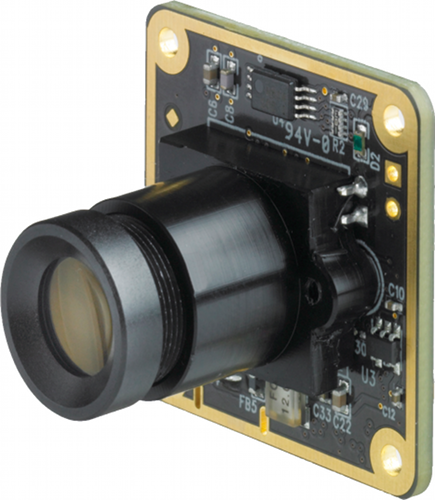
\includegraphics[width=0.4\textwidth, height=0.25\textwidth]{Figures/cam.png}
\caption{\\Left: SparkFun 6DOF IMU. Photo by SparkFun. Adapted from~\cite{create}. Right: The Imaging Source 22BUC03-ML CMOS board camera. Adapted from~\cite{imsrc}}
\label{fig:imu}
%\end{center}
\end{figure}
%%%%%%%%%%%%%%%%%%%%%%%%%%%%%%%%%%%%%%%%%%%%%%%%%%%%%%%%%%%%%%%%%%%%%%%%%%
\subsubsection{CMOS Machine Vision Camera}
The measurement sensor is required to be a single camera. The problem description only requires the camera to have a 30 Hz frame rate. The camera chosen for this project is a CMOS camera by The Imaging Source as depicted in Figure~\ref{fig:imu}. The DFM 22BUC03-ML model is a machine vision board contains 4 GPIO pins that allow the shutter to be triggered. The camera was used for a previous project and incorporated in this project due to cost constrains.\\\\ 
The camera is configured with the following properties:
\begin{itemize}
\item Trigger mode, receiving a pulse to sample a frame (typically 30 Hz).
\item Monochrome image capture (for efficiency).
\end{itemize}

The \textit{intrinsic} matrix of the camera in Equation~\ref{eq:fmmd1} and the distortion coefficients are determined through camera calibration made available by OpenCV~\cite{opencv}. The results of this procedure are given as follows:

\begin{table}[H]
\caption{Intrinsic and distortion camera parameters}
\begin{center}
\begin{tabular}{|c|c|}
\hline
Parameter & Values \\
\hline
focal length $f$ & 1019 pixels \\
\hline
$u_0$& 319 pixels \\
\hline
$v_0$& 241 pixels \\
\hline
Distortion coefficient $K$ &  0.504\\
\hline
\end{tabular}
\end{center}
\label{camval}
\end{table}%

The trigger pulse is set by the micro-controller, this will be discussed next.
%%%%%%%%%%%%%%%%%%%%%%%%%%%%%%%%%%%%%%%%%%%%%%%%%%%%%%%%%%%%%%%%%%%%%%%%%%
\subsubsection{Micro-controller}
A micro-controller is required for two reasons. Firstly, the values received from the IMU are analog and need to be converted to digital. Secondly, the camera is configured to receive a pulse to capture a frame. This pulse needs to be sent by the Arduino every sampling instance and simultaneously sample the IMU data so that the image data and the IMU data remain \textit{synchronised}.

\begin{figure}[htbp]
\begin{center}
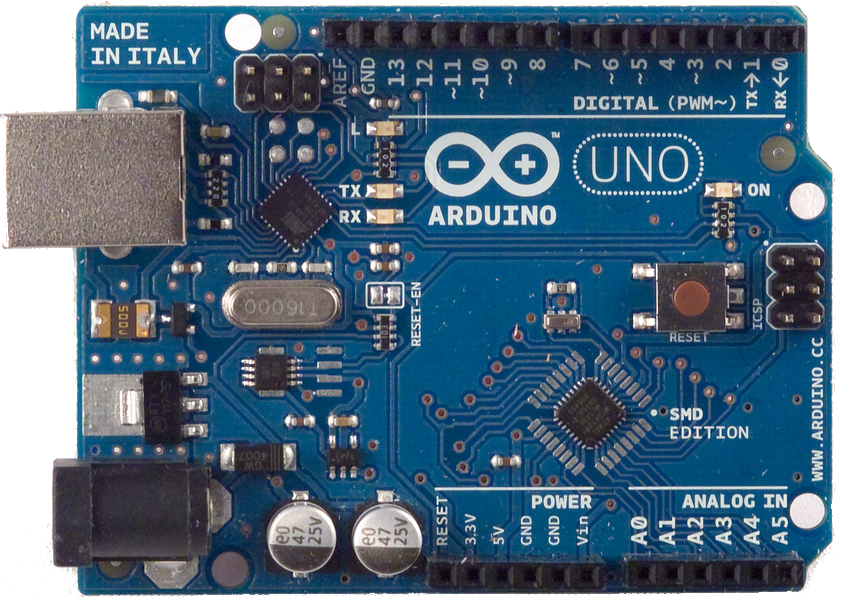
\includegraphics[width=0.5\textwidth, height=0.3\textwidth]{Figures/arduino.jpg}
\caption{Arduino UNO SMD by Arduino. Adapted from~\cite{create}.}
\label{fig:arduno}
\end{center}
\end{figure}
%%%%%%%%%%%%%%%%%%%%%%%%%%%%%%%%%%%%%%%%%%%%%%%%%%%%%%%%%%%%%%%%%%%%%%%%%%

This project doesn't require a large micro-controller. The specifications for the micro-controller are shown as follows:
\begin{itemize}
\item Two A2D ports for I2C communication with the IMU.
\item 3.3 Volt supply voltage for the IMU.
\item One digital output pin to trigger a pulse to the camera.
\item Support community.
\end{itemize}

The Arduino micro-controllers provide a suitable, low cost solution. The Arduino Uno SMD Rev3~\cite{arduino} in particular is a scaled down version of the original Uno, providing the necessary functionality along with a helpful developer community with many forums and available code segments for the IMU used in this project. 
%\subsection{Design Choices}

%\subsubsection{Serial Communication}
%\begin{table}[H]
%\caption{Single-Byte I2C Write Cycle}
%\begin{center}
%\begin{tabular}{|c|c|c|c|c|c|c|c|c|}
%\hline
%master & start & device adr + write & & register adr & & data & & stop \\ 
%\hline
%slave & & & ack & & ack & & ack &  \\
%\hline
%\end{tabular}
%\end{center}
%\label{tab:read}
%\end{table}
%\begin{table}[H]
%\caption{Single-Byte I2C Read Cycle}
%\begin{center}
%\begin{tabular}{|c|c|c|c|c|c|c|c|c|c|c|c|}
%\hline
%master & start & device add & & register adr & & start & register adr & & & $\overline{\text{ack}}$ & stop \\ 
%\hline
%slave& & & ack & & ack & & & ack & data &  &\\
%\hline
%\end{tabular}
%\end{center}
%\label{tab:write}
%\end{table}
%%%%%%%%%%%%%%%%%%%%%%%%%%%%%%%%%%%%%%%%%%%%%%%%%%%%%%%%%%%%%%%%%%%%%%%%%%
%\subsubsection{}
%%%%%%%%%%%%%%%%%%%%%%%%%%%%%%%%%%%%%%%%%%%%%%%%%%%%%%%%%%%%%%%%%%%%%%%%%%
\newpage
\subsection{Simulation}
This study seeks to investigate the performance of the kinematic estimator as a state transition model. An EKF-based kinematic estimator simulation is designed to meet the following specifications:
\begin{itemize}
\item The measurement update only adds additive noise to the state estimates. 
\item The kinematic estimator should precisely track a trajectory of a robot from simulated IMU measurements, given that there is no uncertainty regarding the system.
\item In the event of process and measurement noise, the kinematic estimator should still allow the EKF provide an optimal estimate depending on the amount of uncertainty each noise perturbation presents.  
\end{itemize}

In order to effectively analyse it's performance, a simulation of an EKF that uses a kinematic estimator as the state transition model is run under a set of test conditions. These conditions will accurately analyse the performance of the kinematic estimator with regard to the aforementioned design specifications. A functional diagram of the EKF-based kinematic estimator (based on Equation~\ref{eq:trmod}) is shown in Figure~\ref{fig:kindiag}. The kinematic estimator is incorporated within the control update of the EKF. %A set of \textit{simulated} inertial measurements will initially be inserted into the kinematic estimator simulation and the resulting trajectory will be plotted to provide better insight. Thereafter a set of random measurements will be inserted into the kinematic estimator with  
\begin{figure}[htbp]
\begin{center}
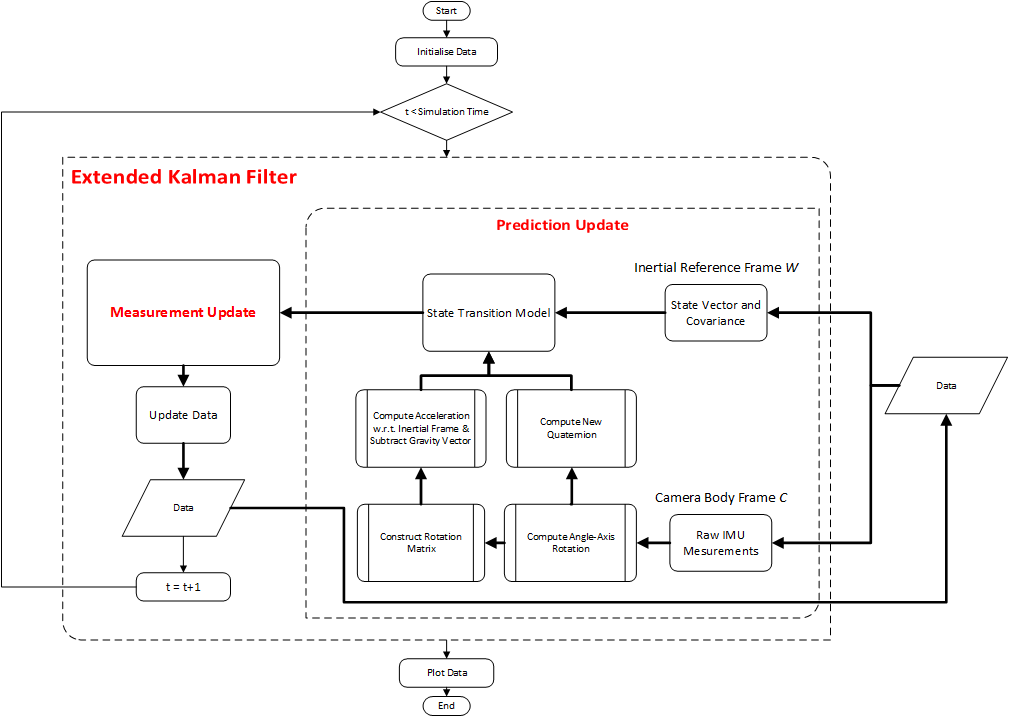
\includegraphics[width=\textwidth, height=0.8\textwidth]{Figures/Drawing3.png}
\caption{EKF using a kinematic estimator to provide the control update.}
\label{fig:kindiag}
\end{center}
\end{figure}

\newpage
\subsubsection{Test 1: Prediction}
The first set of test conditions will provide simulated gyroscope and accelerometer measurements with zero process and measurement noise. The EKF simulation measurement model is defined as a mapping of the state vector with additive noise. With no uncertainty regarding the measurement or process noise then, the simulated state estimates should exactly resemble the actual state vector.

The expected outcome then, is that the kinematic estimator will precisely track a given robot trajectory. These trajectories will be trivially defined so that the results can be accurately analysed. 
\\\\
The first set of test conditions as well as the theoretical predictions are given as follows 
It is worthwhile to note that the length of a simulation is 10 seconds at 30 Hz or 300 samples. The initial position is always $\textbf{r}^W$ = \{0 0 0\} with an orientation quaternion of $\textbf{q}^{WC} =$ \{1 0 0 0\}): %The trajectory of the can thus qualitatively analysed to predict the performance of the kinematic estimato.

\begin{enumerate}
\item \textbf{1 metre per second x-acceleration:}\\
The trajectory is expected to only move along the positive x-axis. Newtons equations of motions suggest that the displacement of the robot due to a constant acceleration is:
\begin{equation}
x = x_0 + \cfrac{t^2}{2} = 0 + \cfrac{10^2}{2} = 50 \text{m}
\end{equation}
\item \textbf{1 metre per second x-acceleration with sudden positive 90 degree rotation about the y-axis:}\\
The trajectory is expected to initially move along the positive x-axis after which the positive 90 degree rotation about the y-axis will rotate the robot frame so that the trajectory only moves along the negative z-axis. 
\item \textbf{1 metre per second x-acceleration with three consecutive 90 degree rotations about the z-axis:}\\
The trajectory is expected to initially move along the positive x-axis until the first positive 90 degree rotation about the z-axis rotates the robot frame so that the trajectory only moves along the positive y-axis. A second positive 90 degree rotation about the z-axis rotates the robot frame so that the trajectory then moves along the negative x-axis. The final positive 90 degree rotation about the z-axis rotates the robot frame so that the trajectory only moves along the negative y-axis. If the time-steps between the rotations are equal, a block figure trajectory is expected in the plane of rotation.    
\end{enumerate}
\newpage
\subsubsection{Test 1: Results and Analysis}
\begin{enumerate}
\item \textbf{1 metre per second x-acceleration:}\\
The simulation depicted in Figure~\ref{fig:xacc} shows a trajectory only moving along the positive x-axis. The final x-position is given to be 50 metres, exactly the predicted value. Furthermore, the estimated trajectory directly tracks the true trajectory.  
\item  \textbf{1 metre per second x-acceleration with sudden 90 degree rotation about the y-axis:}\\
The simulation depicted in Figure~\ref{fig:yrot} shows a trajectory that initially moves along the positive x-axis before proceeding to move along the negative z-axis. Again, the estimated trajectory directly tracks the true trajectory.
\item  \textbf{1 metre per second x-acceleration with three consecutive 90 degree rotations about the z-axis:}\\   
The simulation depicted in Figure~\ref{fig:zplane} shows a square in the z-plane. This suggests that the trajectory incorporates three 90 degree rotations about the z-axis as the robot is moving at a constant acceleration with respect to its own reference frame. Again, the estimated trajectory directly tracks the true trajectory.

\end{enumerate}
\begin{figure}[H]
%\centering
\begin{subfigure}[H]{0.49\textwidth}
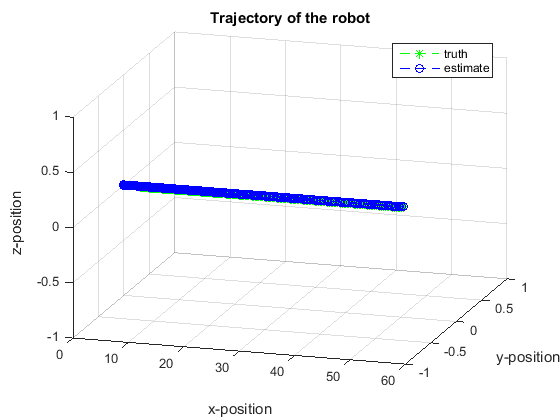
\includegraphics[width=\textwidth, height=5.8cm]{Figures/accx_1_traj.png} 
\caption{Trajectory: 1 m/s x-acceleration.}
\label{fig:xacc}
\end{subfigure}
\begin{subfigure}[H]{0.49\textwidth}
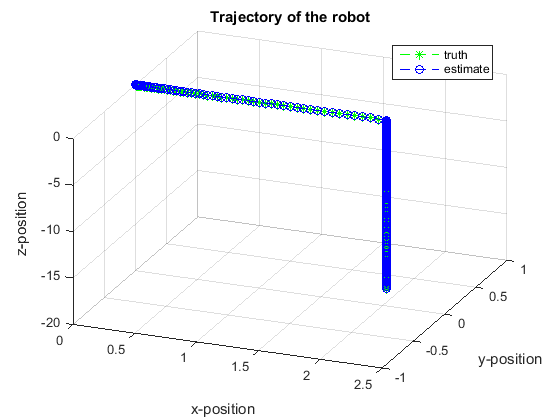
\includegraphics[width=\textwidth, height=5.8cm]{Figures/90rotx_traj.png}
\caption{Trajectory: 1 m/s x-acceleration with sudden $90^{\circ}$ rotation about the y-axis.}
\label{fig:yrot}
\end{subfigure}
\begin{subfigure}[H]{0.49\textwidth}
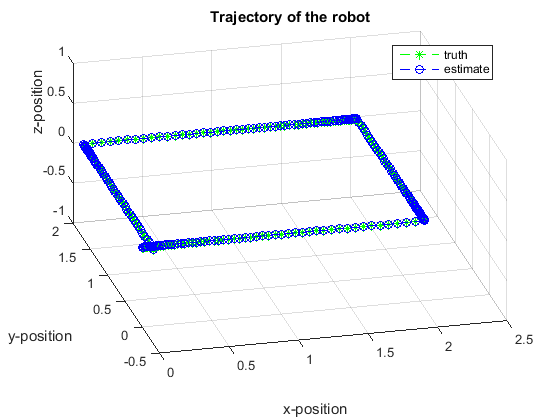
\includegraphics[width=\textwidth, height=5.8cm]{Figures/xy_block_traj.png}
\caption{Trajectory: 1 m/s x-acceleration with three consecutive $90^{\circ}$ rotations about the z-axis.}
\label{fig:zplane}
\end{subfigure} 
\caption{Results of the test conditions 1 depicting zero-uncertainty.}
\label{fig:sim1}
\end{figure}
%%%%%%%%%%%%%%%%%%%%%%%%%%%%%%%%%%%%%%%%%%%%%%%%%%%%%%%%%%%%%%%%%%%%%%%%%%
\subsubsection{Test 2: Prediction}
The second set of test conditions will provide \textit{randomly} simulated gyroscope and accelerometer measurements \textbf{with} simulated process and measurement noise. The EKF simulation measurement model is still defined as a mapping of the state vector with additive noise. The EKF should now behave as described in Chapter~\ref{sec:EKF} while maintaining the performance of the kinematic state estimator. 

The expected outcome then, is that the kinematic estimator will track the given robot trajectory according to the uncertainty of both the measurement and process noise. Intuitively, the EKF should provide a state estimate that is dependent upon the process and measurement noise e.g. it the system has a high measurement noise uncertainty but a low process noise uncertainty, the EKF should provide a state estimate that depends less on the measurements.       

\begin{enumerate}
\item  \textbf{No uncertainty: Process noise variance = 0 and Measurement noise variance = 0}\\
This trajectory estimate is expected to precisely resemble the true trajectory as there is no uncertainty regarding the measurement nor the process noise.
\item  \textbf{Equal yet small uncertainty regarding the measurement and process noise}\\
The EKF is expected to provide a trajectory estimate that incorporates both the measurements and the equivalent control inputs (IMU measurements) but still reasonable approximate the true trajectory due to the small uncertainty.   
\item  \textbf{Equal yet high uncertainty regarding the measurement and process noise}\\   
The EKF is expected to provide a trajectory estimate that again incorporates both the measurements and the equivalent control inputs. The trajectory estimate however, will vastly differ from the true trajectory due to the high uncertainty. 
\item  \textbf{Less certain process noise: Process noise variance = large and measurement noise variance = small}\\   
The EKF is expected to provide a trajectory estimate that is more reliant upon the measurements as it incorporates less uncertainty than the equivalent control inputs. Provided that the measurement noise is small enough, the EKF should still provide a reasonable approximation of the true trajectory.
\end{enumerate}
\subsubsection{Test 2: Results and Analysis}
\begin{enumerate}
\item  \textbf{No uncertainty: Process noise variance = 0 and measurement noise variance = 0}\\
This simulation depicted in Figure~\ref{fig:notraj} shows a trajectory estimate that directly resembles the true trajectory. This is due to the fact that there is no uncertainty regarding the process or the measurement noise and the EKF can accurately estimate the actual state of the system through modelling. Figure~\ref{fig:noz} confirms that both the measurements and estimates agree are in correspondence with the states. This particular case though is only possible in simulation and practically impossible as every practical system incorporates uncertainty.   
\item  \textbf{Equal yet small uncertainty regarding the measurement and process noise}\\
This simulation depicted in Figure~\ref{fig:equaltraj} shows a trajectory estimate that is noisy but generally tracks the actual trajectory. This behaviour corresponds to the aforementioned prediction that the EKF is not entirely certain regarding both the measurements and equivalent control inputs and subsequently provides an estimate that incorporates information from both factors. Figure~\ref{fig:equalz} shows that the state estimate incorporates uncertainty regarding both the measurements and the equivalent control inputs. Because these uncertainties are small though, a relatively accurate reconstruction of the actual trajectory can be estimated.     
\item  \textbf{Less certain process noise: Process noise variance = large and measurement noise variance = small}\\   
 This simulation depicted in Figures~\ref{fig:high_traj} and~\ref{fig:xhigh} shows a trajectory estimate that doesn't resemble the true trajectory. This is due to the fact that the EKF ``trusts" the information it receives and if this information is very uncertain, the EKF still provides the best estimate given the information, but even that estimate is very wrong. The quality of the information provided to the EKF is thus critical.  
\item  \textbf{Less certain process noise: Process noise variance = large and measurement noise variance = small}\\   
This simulation depicted in Figure~\ref{fig:meastraj} shows a trajectory estimate that is noisy and heavily incorporates the measurements. This behaviour corresponds to the aforementioned prediction that the EKF very uncertain regarding the equivalent control inputs and subsequently provides an estimate that incorporates more information from measurements. Figure~\ref{fig:equalz} shows that the state estimate incorporates more information regarding the measurements. Because the measurement uncertainty isn't very small, the EKF cannot provide an accurate approximation of the true trajectory. This is due to the fact that the EKF ``trusts" the measurements far more than the equivalent control inputs, but because the measurements themselves contain a substantial amount of uncertainty, the best estimate that the EKF can provide is itself uncertain.  
\end{enumerate}
\begin{figure}[h]
%\centering
\begin{subfigure}[H]{0.49\textwidth}
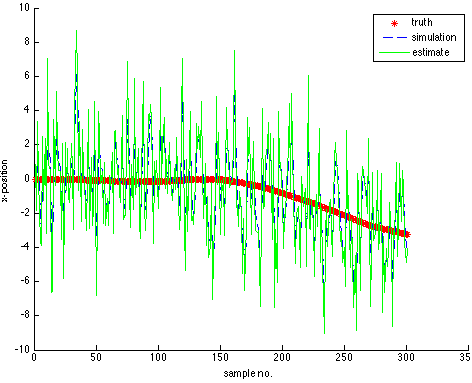
\includegraphics[width=\textwidth, height=6cm]{Figures/xhigh.png}
\caption{X-position of random control inputs with equally high process and measurement uncertainty.}
\label{fig:xhigh}
\end{subfigure}
\begin{subfigure}[H]{0.49\textwidth}
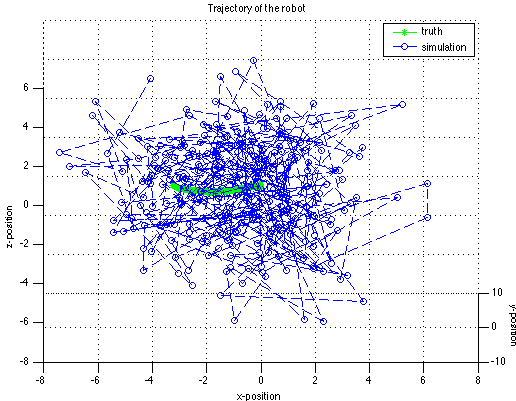
\includegraphics[width=\textwidth, height=6cm]{Figures/high_traj.png} 
\caption{Trajectory of random control inputs with equally high process and measurement uncertainty.}
\label{fig:high_traj}
\end{subfigure}
\label{fig:extra}
\caption{Results of the conditions depicting random equivalent control inputs with uncertainty.}
\end{figure}

\begin{figure}[H]
%\centering
\begin{subfigure}[H]{0.49\textwidth}
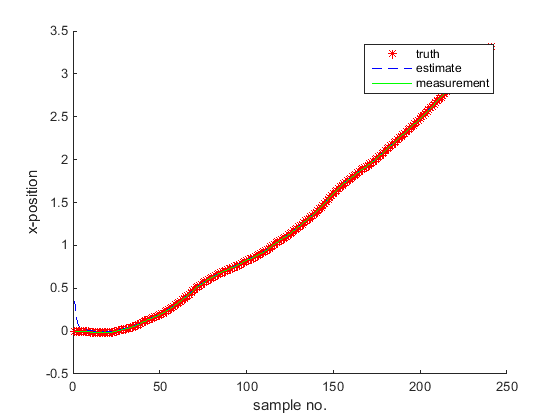
\includegraphics[width=\textwidth, height=6.4cm]{Figures/kf_none_x.png} 
\caption{X-position of random control inputs with zero-uncertainty.}
\label{fig:noz}
\end{subfigure}
\begin{subfigure}[H]{0.49\textwidth}
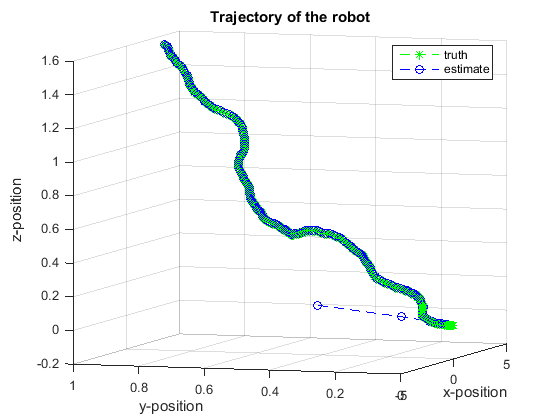
\includegraphics[width=\textwidth, height=6.4cm]{Figures/kf_none_traj.png}
\caption{Trajectory of random control inputs with zero-uncertainty.}
\label{fig:notraj}
\end{subfigure}
\begin{subfigure}[H]{0.49\textwidth}
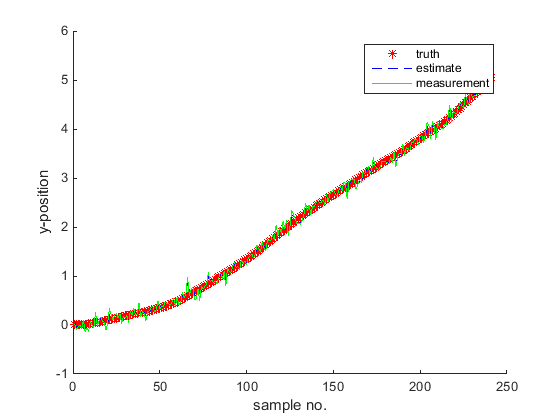
\includegraphics[width=\textwidth, height=6.5cm]{Figures/kf_eq001_y.png}
\caption{Y-position of random control inputs with a small, equal measurement and process uncertainty.}
\label{fig:equalz}
\end{subfigure} 
\begin{subfigure}[H]{0.49\textwidth}
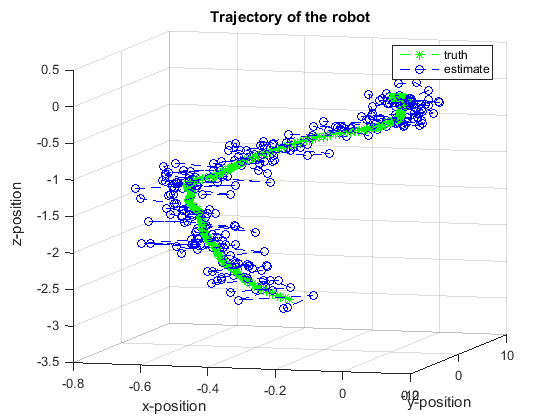
\includegraphics[width=\textwidth, height=6.5cm]{Figures/kf_eq001_traj.png}
\caption{Trajectory of random control inputs with a small, equal measurement and process uncertainty.}
\label{fig:equaltraj}
\end{subfigure} 
\begin{subfigure}[H]{0.49\textwidth}
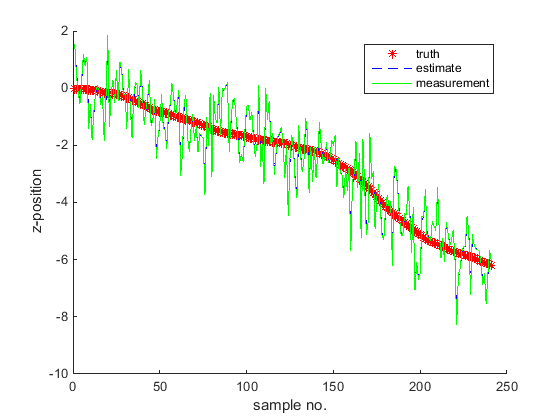
\includegraphics[width=\textwidth, height=6.5cm]{Figures/kf_pro10to1_z.png}
\caption{Z-position of random control inputs with greater process uncertainty.}
\label{fig:measz}
\end{subfigure} 
\begin{subfigure}[H]{0.49\textwidth}
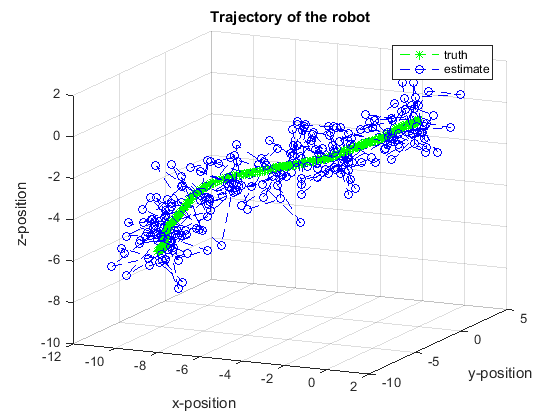
\includegraphics[width=\textwidth, height=6.5cm]{Figures/kf_pro10to1_traj.png}
\caption{Trajectory of random control inputs with greater process uncertainty.}
\label{fig:meastraj}
\end{subfigure}
\caption{Results of the conditions depicting random equivalent control inputs with uncertainty.}
\label{fig:sim1}
\end{figure}
%%%%%%%%%%%%%%%%%%%%%%%%%%%%%%%%%%%%%%%%%%%%%%%%%%%%%%%%%%%%%%%%%%%%%%%%%%
%%%%%%%%%%%%%%%%%%%%%%%%%%%%%%%%%%%%%%%%%%%%%%%%%%%%%%%%%%%%%%%%%%%%%%%%%%
%%%%%%%%%%%%%%%%%%%%%%%%%%%%%%%%%%%%%%%%%%%%%%%%%%%%%%%%%%%%%%%%%%%%%%%%%%
%%%%%%%%%%%%%%%%%%%%%%%%%%%%%%%%%%%%%%%%%%%%%%%%%%%%%%%%%%%%%%%%%%%%%%%%%%
%%%%%%%%%%%%%%%%%%%%%%%%%%%%%%%%%%%%%%%%%%%%%%%%%%%%%%%%%%%%%%%%%%%%%%%%%%
\newpage
\section{Analysis: Testing \& Results}
%%%%%%%%%%%%%%%%%%%%%%%%%%%%%%%%%%%%%%%%%%%%%%%%%%%%%%%%%%%%%%%%%%%%%%%%%%
%%%%%%%%%%%%%%%%%%%%%%%%%%%%%%%%%%%%%%%%%%%%%%%%%%%%%%%%%%%%%%%%%%%%%%%%%%
%%%%%%%%%%%%%%%%%%%%%%%%%%%%%%%%%%%%%%%%%%%%%%%%%%%%%%%%%%%%%%%%%%%%%%%%%%
%%%%%%%%%%%%%%%%%%%%%%%%%%%%%%%%%%%%%%%%%%%%%%%%%%%%%%%%%%%%%%%%%%%%%%%%%%
%%%%%%%%%%%%%%%%%%%%%%%%%%%%%%%%%%%%%%%%%%%%%%%%%%%%%%%%%%%%%%%%%%%%%%%%%%
%%%%%%%%%%%%%%%%%%%%%%%%%%%%%%%%%%%%%%%%%%%%%%%%%%%%%%%%%%%%%%%%%%%%%%%%%%
%%%%%%%%%%%%%%%%%%%%%%%%%%%%%%%%%%%%%%%%%%%%%%%%%%%%%%%%%%%%%%%%%%%%%%%%%%
%%%%%%%%%%%%%%%%%%%%%%%%%%%%%%%%%%%%%%%%%%%%%%%%%%%%%%%%%%%%%%%%%%%%%%%%%%
%%%%%%%%%%%%%%%%%%%%%%%%%%%%%%%%%%%%%%%%%%%%%%%%%%%%%%%%%%%%%%%%%%%%%%%%%%
%%%%%%%%%%%%%%%%%%%%%%%%%%%%%%%%%%%%%%%%%%%%%%%%%%%%%%%%%%%%%%%%%%%%%%%%%%
%%%%%%%%%%%%%%%%%%%%%%%%%%%%%%%%%%%%%%%%%%%%%%%%%%%%%%%%%%%%%%%%%%%%%%%%%%
%%%%%%%%%%%%%%%%%%%%%%%%%%%%%%%%%%%%%%%%%%%%%%%%%%%%%%%%%%%%%%%%%%%%%%%%%%
%%%%%%%%%%%%%%%%%%%%%%%%%%%%%%%%%%%%%%%%%%%%%%%%%%%%%%%%%%%%%%%%%%%%%%%%%%
%%%%%%%%%%%%%%%%%%%%%%%%%%%%%%%%%%%%%%%%%%%%%%%%%%%%%%%%%%%%%%%%%%%%%%%%%%
%%%%%%%%%%%%%%%%%%%%%%%%%%%%%%%%%%%%%%%%%%%%%%%%%%%%%%%%%%%%%%%%%%%%%%%%%%
%%%%%%%%%%%%%%%%%%%%%%%%%%%%%%%%%%%%%%%%%%%%%%%%%%%%%%%%%%%%%%%%%%%%%%%%%%
%%%%%%%%%%%%%%%%%%%%%%%%%%%%%%%%%%%%%%%%%%%%%%%%%%%%%%%%%%%%%%%%%%%%%%%%%%
%%%%%%%%%%%%%%%%%%%%%%%%%%%%%%%%%%%%%%%%%%%%%%%%%%%%%%%%%%%%%%%%%%%%%%%%%%
%%%%%%%%%%%%%%%%%%%%%%%%%%%%%%%%%%%%%%%%%%%%%%%%%%%%%%%%%%%%%%%%%%%%%%%%%%
%%%%%%%%%%%%%%%%%%%%%%%%%%%%%%%%%%%%%%%%%%%%%%%%%%%%%%%%%%%%%%%%%%%%%%%%%%
%%%%%%%%%%%%%%%%%%%%%%%%%%%%%%%%%%%%%%%%%%%%%%%%%%%%%%%%%%%%%%%%%%%%%%%%%%
%%%%%%%%%%%%%%%%%%%%%%%%%%%%%%%%%%%%%%%%%%%%%%%%%%%%%%%%%%%%%%%%%%%%%%%%%%
%%%%%%%%%%%%%%%%%%%%%%%%%%%%%%%%%%%%%%%%%%%%%%%%%%%%%%%%%%%%%%%%%%%%%%%%%%
%%%%%%%%%%%%%%%%%%%%%%%%%%%%%%%%%%%%%%%%%%%%%%%%%%%%%%%%%%%%%%%%%%%%%%%%%%
%%%%%%%%%%%%%%%%%%%%%%%%%%%%%%%%%%%%%%%%%%%%%%%%%%%%%%%%%%%%%%%%%%%%%%%%%%
%%%%%%%%%%%%%%%%%%%%%%%%%%%%%%%%%%%%%%%%%%%%%%%%%%%%%%%%%%%%%%%%%%%%%%%%%%
%%%%%%%%%%%%%%%%%%%%%%%%%%%%%%%%%%%%%%%%%%%%%%%%%%%%%%%%%%%%%%%%%%%%%%%%%%
%%%%%%%%%%%%%%%%%%%%%%%%%%%%%%%%%%%%%%%%%%%%%%%%%%%%%%%%%%%%%%%%%%%%%%%%%%
%%%%%%%%%%%%%%%%%%%%%%%%%%%%%%%%%%%%%%%%%%%%%%%%%%%%%%%%%%%%%%%%%%%%%%%%%%
%%%%%%%%%%%%%%%%%%%%%%%%%%%%%%%%%%%%%%%%%%%%%%%%%%%%%%%%%%%%%%%%%%%%%%%%%%
%%%%%%%%%%%%%%%%%%%%%%%%%%%%%%%%%%%%%%%%%%%%%%%%%%%%%%%%%%%%%%%%%%%%%%%%%%
%%%%%%%%%%%%%%%%%%%%%%%%%%%%%%%%%%%%%%%%%%%%%%%%%%%%%%%%%%%%%%%%%%%%%%%%%%
%%%%%%%%%%%%%%%%%%%%%%%%%%%%%%%%%%%%%%%%%%%%%%%%%%%%%%%%%%%%%%%%%%%%%%%%%%
%%%%%%%%%%%%%%%%%%%%%%%%%%%%%%%%%%%%%%%%%%%%%%%%%%%%%%%%%%%%%%%%%%%%%%%%%%
%%%%%%%%%%%%%%%%%%%%%%%%%%%%%%%%%%%%%%%%%%%%%%%%%%%%%%%%%%%%%%%%%%%%%%%%%%
%%%%%%%%%%%%%%%%%%%%%%%%%%%%%%%%%%%%%%%%%%%%%%%%%%%%%%%%%%%%%%%%%%%%%%%%%%
%%%%%%%%%%%%%%%%%%%%%%%%%%%%%%%%%%%%%%%%%%%%%%%%%%%%%%%%%%%%%%%%%%%%%%%%%%
%%%%%%%%%%%%%%%%%%%%%%%%%%%%%%%%%%%%%%%%%%%%%%%%%%%%%%%%%%%%%%%%%%%%%%%%%%
%%%%%%%%%%%%%%%%%%%%%%%%%%%%%%%%%%%%%%%%%%%%%%%%%%%%%%%%%%%%%%%%%%%%%%%%%%
%%%%%%%%%%%%%%%%%%%%%%%%%%%%%%%%%%%%%%%%%%%%%%%%%%%%%%%%%%%%%%%%%%%%%%%%%%
%%%%%%%%%%%%%%%%%%%%%%%%%%%%%%%%%%%%%%%%%%%%%%%%%%%%%%%%%%%%%%%%%%%%%%%%%%
%%%%%%%%%%%%%%%%%%%%%%%%%%%%%%%%%%%%%%%%%%%%%%%%%%%%%%%%%%%%%%%%%%%%%%%%%%
%%%%%%%%%%%%%%%%%%%%%%%%%%%%%%%%%%%%%%%%%%%%%%%%%%%%%%%%%%%%%%%%%%%%%%%%%%
%%%%%%%%%%%%%%%%%%%%%%%%%%%%%%%%%%%%%%%%%%%%%%%%%%%%%%%%%%%%%%%%%%%%%%%%%%
%%%%%%%%%%%%%%%%%%%%%%%%%%%%%%%%%%%%%%%%%%%%%%%%%%%%%%%%%%%%%%%%%%%%%%%%%%
%%%%%%%%%%%%%%%%%%%%%%%%%%%%%%%%%%%%%%%%%%%%%%%%%%%%%%%%%%%%%%%%%%%%%%%%%%
%%%%%%%%%%%%%%%%%%%%%%%%%%%%%%%%%%%%%%%%%%%%%%%%%%%%%%%%%%%%%%%%%%%%%%%%%%
%%%%%%%%%%%%%%%%%%%%%%%%%%%%%%%%%%%%%%%%%%%%%%%%%%%%%%%%%%%%%%%%%%%%%%%%%%
%%%%%%%%%%%%%%%%%%%%%%%%%%%%%%%%%%%%%%%%%%%%%%%%%%%%%%%%%%%%%%%%%%%%%%%%%%
%%%%%%%%%%%%%%%%%%%%%%%%%%%%%%%%%%%%%%%%%%%%%%%%%%%%%%%%%%%%%%%%%%%%%%%%%%













%%%%%%%%%%%%%%%%%%%%%%%%%%%%%%%%%%%%%%%%%%%%%%%%%%%%%%%%%%%%%%%%%%%%%%%%%%

\newpage
%\pagenumbering{roman}
\appendix
\section{Summary of Work done}
\newpage
%%%%%%%%%%%%%%%%%%%%%%%%%%%%%%%%%%%%%%%%%%%%%%%%%%%%%%%%%%%%%%%%%%%%%%%%%%
\section{Achieved ECSA Exit Level Outcomes}
\newpage
%%%%%%%%%%%%%%%%%%%%%%%%%%%%%%%%%%%%%%%%%%%%%%%%%%%%%%%%%%%%%%%%%%%%%%%%%%

%%%%%%%%%%%%%%%%%%%%%%%%%%%%%%%%%%%%%%%%%%%%%%%%%%%%%%%%%%%%%%%%%%%%%%%%%%
\section{Theoretical Concepts} \label{App:Concepts}
\subsection{State Space Model} 
As previously discussed, the EKF requires a state transition model in order to estimate the current state of the system. In short, the motion model describes the transition from the previous state to the following state with regard to the robot's kinematic motion as well as the control inputs. The \textit{ideal} motion model in this particular instance can be described through a \textbf{linear} differential equation of the following form:
\begin{equation}
\textbf{\.{x}}_t = \textbf{A}\textbf{x}_{t-1} + \textbf{B}\textbf{u}_t+\textbf{w}_t,
\end{equation} 
where the state matrix $\textbf{A}$, describes the manner in which state evolves from the previous time-step to the current time-step without the influence of noise and controls, the input matrix $\textbf{B}$, describes how the control vector $\textbf{u}_t$ evolves from the previous time-step to the current time-step and $\textbf{w}_t$ is a \textbf{zero-mean} Gaussian process representing the process noise with a covariance matrix $\textbf{R}_w$.\\\\
Considering that the EKF is a recursive, numerical evaluation, it is necessary to convert the previously defined continuous model into its discrete counterpart. Various methods of discretisation exist, though this specific implementation makes use of the forward difference/Euler�s method. This method  \textit{approximates} the derivative for a state for a sampling period $\Delta T$ as follows:  
\begin{equation}
\begin{split}
\textbf{\.{x}}_k &= \lim_{\Delta T\to 0}{\frac{\textbf{x}_{k+1}-\textbf{x}_k}{\Delta T}} 		 \\										\Delta T\textbf{\.{x}}_k &\approx \textbf{x}_{k+1}-\textbf{x}_k, \\
\end{split}
\end{equation}     
The state estimate of the discrete counterpart at the following sampling instance, namely $k + 1$, is then presented as follows (given a small enough sampling instance $\Delta T$):
\begin{equation}
\begin{split}
\textbf{x}_{k+1} &= \big(\textbf{I}+\textbf{A}\Delta T\big)\textbf{x}_k + \textbf{B}\textbf{u}_k\Delta T + \textbf{w}_k\Delta T,
\end{split}
\end{equation}
where $\big(\textbf{I}+\textbf{A}\Delta T\big) = \textbf{A}_d$ is the discrete state matrix, $ \textbf{B}\Delta T = \textbf{B}_d$ is the discrete input matrix and $\textbf{w}_k\Delta T=\textbf{w}_{d,k}$ is the discrete input process noise. \\\\
Ultimately, the form of the final difference equation describing the system at each individual sampling instance is given as follows:
\begin{equation}
\textbf{x}_{k+1}= \textbf{A}_d\textbf{x}_k + \textbf{B}_d\textbf{u}_k+\textbf{w}_{d,k},
\end{equation} 
%%%%%%%%%%%%%%%%%%%%%%%%%%%%%%%%%%%%%%%%%%%%%%%%%%%%%%%%%%%%%%%%%%%%%%%%%%
\subsection{State Transition: Linear Model}
In order to derive the motion model for the system at hand, it is vital that the certain characteristics of the system be understood. Firstly, the robot system is comprised of a monocular camera and an attached IMU package. Secondly, the camera is to be considered as a 6 DOF rigid body. Briefly the six DOF describe the camera's three \textit{translational} and three \textit{rotational} degrees of freedom. \\
We therefore set out to define a kinematic motion model - using Newton's laws of motion - to describe the cameras movement through the environment as a result of initially unknown, external inputs to the system. Lastly, it should be stressed that embedded within the motion model, should be the impacts of uncertainty through both internal and external factors. 
%It is assumed in this instance, that at each time-step, an unknown angular acceleration $\mathbf{\Omega}^R$ acts upon the system. This input is modelled as a zero-mean Gaussian process that causes an impulse of angular velocity:
%\begin{equation}
%\textbf{w}_d[k]  = \textbf{w}[k] \Delta T =     
% \begin{bmatrix}
% \mathbf{\Omega}^R
% \end{bmatrix} = 
%  \begin{pmatrix}
%  	\alpha_x \Delta T \\
% 	\alpha_y \Delta T \\
%\alpha_z \Delta T \\
% \end{pmatrix} .
%\end{equation}  
%with a covariance matrix $\textbf{R}_w$ that is assumed as a diagonal initially, to represent uncorrelated noise in all of the rotational components.\\
%With reference to the previously defined state motion model in (1.8)
It must also be stressed that initially, a stochastic, linear discrete-time model is adopted to approximate the motion model. Using the kinematic equations of linear and angular motion, it is aimed to ultimately and complete the previously defined state space model. We begin by describing all relevant states and control inputs:
\begin{equation}\label{eq:disc}
\begin{split} 
\textbf{x}[k] &= \big[\textit{x}_{k}\hspace{0.25cm}\textit{y}_{k}\hspace{0.25cm}\textit{z}_{k}\hspace{0.25cm}\textit{\.{x}}_{k}\hspace{0.25cm}\textit{\.{y}}_{k}\hspace{0.25cm}\textit{\.{z}}_{k}\hspace{0.05cm}\hspace{0.25cm}\textit{q}_{0,k}\hspace{0.25cm}\textit{q}_{1,k}\hspace{0.25cm}\textit{q}_{2,k}\hspace{0.25cm}\textit{q}_{3,k}\big]^T \\
\textbf{u}[k] &= \big[\hspace{0.1cm}\ddot{x}_{k}\hspace{0.25cm}\ddot{y}_{k}\hspace{0.25cm}\ddot{z}_{k}\hspace{0.25cm}\textit{\.{q}}_{0,k}\hspace{0.25cm}\textit{\.{q}}_{1,k}\hspace{0.25cm}\textit{\.{q}}_{2,k}\hspace{0.25cm}\textit{\.{q}}_{3,k}\big]^T\\
\end{split}
\end{equation}
and extend the discrete-time difference equation describing the system to incorporate the motion model,  
\begin{equation}
\begin{split}
\textbf{x}_{k+1} &= \textbf{A}_d\textbf{x}_k + \textbf{B}_d\textbf{u}_k+\textbf{w}_{d,k}, \\
\textbf{A}_d&= 
 \begin{bmatrix}
  1 & 0 & 0 & \Delta T & 0 & 0 & 0 & 0 & 0 & 0 \\
  0 & 1 & 0 & 0 & \Delta T & 0 & 0 & 0 & 0 & 0 \\
  0 & 0 & 1 & 0 & 0 & \Delta T & 0 & 0 & 0 & 0 \\
  0 & 0 & 0 & 1 & 0 & 0 & 0 & 0 & 0 & 0 \\
  0 & 0 & 0 & 0 & 1 & 0 & 0 & 0 & 0 & 0 \\
  0 & 0 & 0 & 0 & 0 & 1 & 0 & 0 & 0 & 0 \\
  0 & 0 & 0 & 0 & 0 & 0 & 1 & 0 & 0 & 0 \\
  0 & 0 & 0 & 0 & 0 & 0 & 0 & 1 & 0 & 0 \\
  0 & 0 & 0 & 0 & 0 & 0 & 0 & 0 & 1 & 0 \\
  0 & 0 & 0 & 0 & 0 & 0 & 0 & 0 & 0 & 1 \\
 \end{bmatrix} = (\textbf{I}+\textbf{A}\Delta T\big),  \\
 \textbf{B}_d&=
\begin{bmatrix}
  \Delta T & 0 & 0 & 0 & 0 & 0 & 0 \\
  0 & \Delta T & 0 & 0 & 0 & 0 & 0 \\
  0 & 0 & \Delta T & 0 & 0 & 0 & 0 \\
  0 & 0 & 0 & \Delta T & 0 & 0 & 0 \\
  0 & 0 & 0 & 0 & \Delta T & 0 & 0 \\
  0 & 0 & 0 & 0 & 0 & \Delta T & 0 \\
  0 & 0 & 0 & 0 & 0 & 0 & \Delta T \\
\end{bmatrix} = \textbf{B}\Delta T, \\\\
 \textbf{w}_{d,k} &=\mathcal{N}(0,  \textbf{R}_w) =  
 \begin{pmatrix}
 \textbf{n}_{\textbf{a}_t,k} \\
 \textbf{n}_{\omega_t,k} \\
 \end{pmatrix} = \textbf{w}_{d,k} \Delta T, 
 \end{split}
\end{equation}
it can be observed from the model above that the motion model adheres to the forward method of discretisation derived in equation~\ref{eq:disc}. The motion model also adheres to the Markov process assumption, in that it can be completely described through only its transition from the previous state as well as the control inputs.   
\newpage
%%%%%%%%%%%%%%%%%%%%%%%%%%%%%%%%%%%%%%%%%%%%%%%%%%%%%%%%%%%%%%%%%%%%%%%%%%%%%
\section{Figures \& Diagrams}
\subsection{Schematics \& Circuit Diagrams}
\begin{figure}[h]
\begin{center}
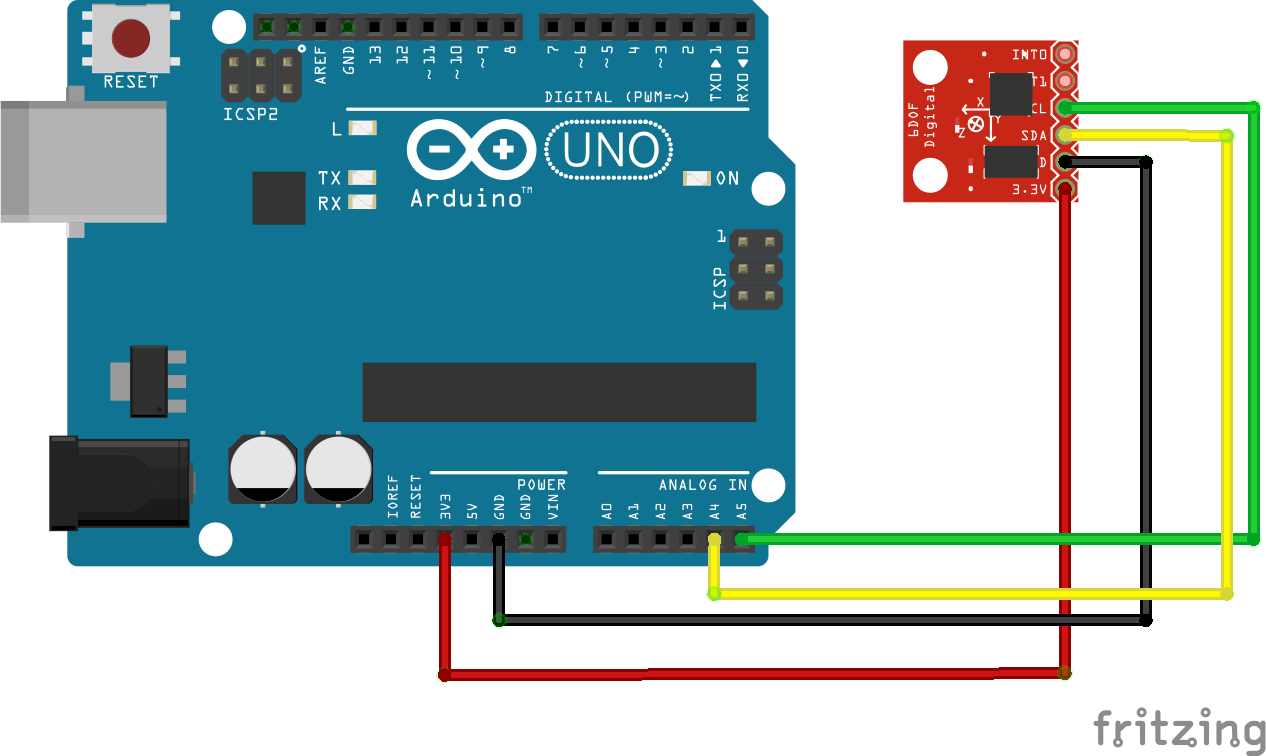
\includegraphics[width=0.8\textwidth, height=0.46\textwidth]{Figures/Schematic_bb.png}
\caption{Circuit Diagram of the IMU.}
\label{fig:circ_dagram}
\end{center}
\end{figure}
\begin{figure}[h]
\begin{center}
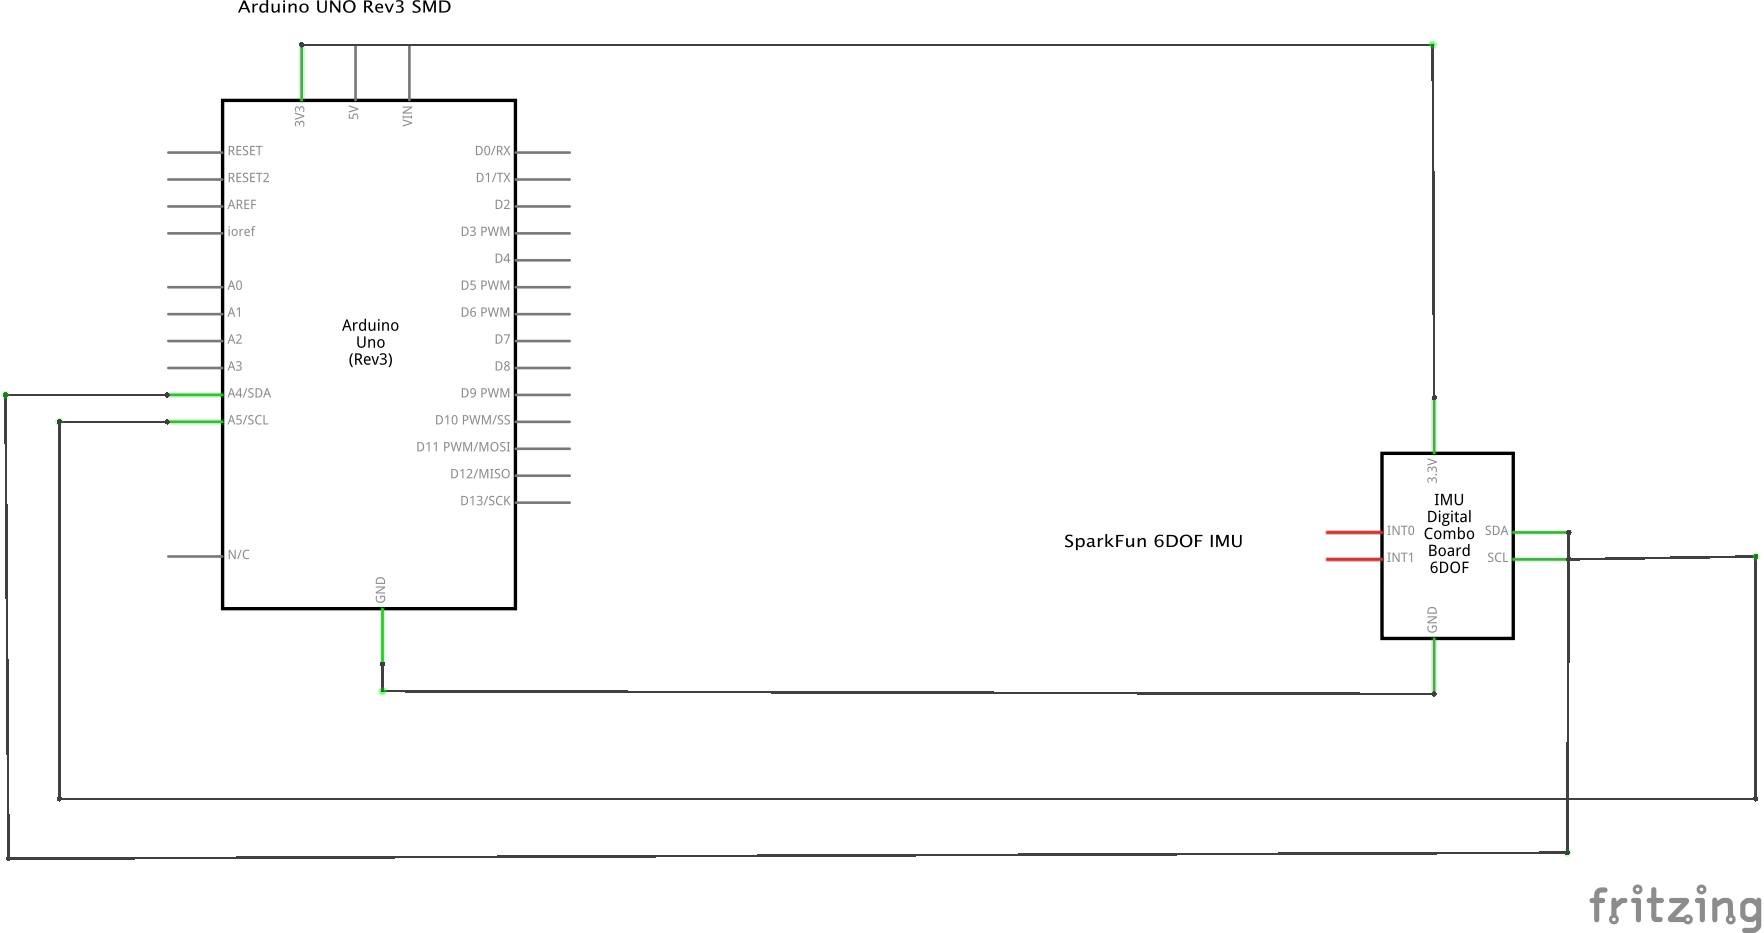
\includegraphics[width=\textwidth, height=0.5\textwidth]{Figures/Schematic.png}
\caption{Schematic of the IMU.}
\label{fig:schematic}
\end{center}
\end{figure}
These images were created by Fritzing (http://fritzing.org)~\cite{create}. 
%\begin{bmatrix}
%x_k\\
%y_k \\ 
%z_k \\
%q_{0,k}\\
%q_{1,k}\\
%q_{2,k}\\
%q_{3,k}\\
%\dot{x}_k\\
%\dot{y}_k\\
%\dot{z}_k\\
%\end{bmatrix}  
%The position state $\textbf{{x}}_p$ can furthermore be fully represented as follows:
%\begin{equation}
%\textbf{{x}}_p=  
% \begin{pmatrix}
% x\\
% y\\ 
% z\\
% q_0\\
% q_1\\
% q_2\\
% q_3\\
% \end{pmatrix} .
%\end{equation}  
%Various alternative implementations exist to represent a robots pose in a 3D space, each presenting their own unique advantages (and disadvantages) with respect to the others. A representation of an arbitrary 3D position and orientation, requires at least, three parameters describing the cartesian position as well as an additional three describing the orientation. This specific implementation, utilises the \textbf{quaternion} representation to portray the orientation information and thus requires an additional parameter to aid its description. 

%This description then allows for the implementation of a recursive algorithm, namely, a discrete KF. In order for a KF to be successfully implemented, a \textbf{state transition (motion) model} as well as an \textbf{observation model} is required to individually describe the effects of the control input as well as the observations respectively.\\
%It is important to note that the KF estimates the state of a continuous- or discrete-time process that is described by a set of differential (continuous) or difference (discrete) equations. The KF then continuously updates the state estimates according to the measurements it obtains. This procedure, takes the form of a two-step recursive process: an a priori prediction (time-update) and an observation based correction (measurement-update). 
\newpage
\bibliographystyle{ieeetr}
\bibliography{Report_bib}
\end{document}   